\listfiles
\documentclass[12pt, letterpaper, ]{report}
\usepackage[style=authoryear, maxnames=2, maxbibnames=99, citestyle=apa]{biblatex}
\addbibresource{merged_biblio2.bib}
\addbibresource{internet_stuff.bib}
%\addbibresource{induction.bib}
%\addbibresource{gwas_silicon.bib}
\usepackage{caption}
\usepackage{geometry}
\usepackage{graphicx}
\usepackage{setspace}
\usepackage{url}
\usepackage{lineno}
\usepackage{tabularx}
\usepackage{gensymb}
\usepackage{longtable}
\usepackage{titlesec}
\usepackage{subcaption}
\usepackage{pdflscape}
\usepackage{booktabs}
\usepackage{array}
\usepackage{fancyhdr}
\pagestyle{fancy}
\fancyhf{}
\fancyfoot[R]{\thepage}
\fancypagestyle{plain}{%
    \renewcommand{\headrulewidth}{0pt}%
    \fancyhf{}%
    \fancyfoot[R]{\thepage}%
}

\newcommand{\mycomment}[1]{}
% Change chapter heading font size to 14pt
\titleformat{\chapter}{\Large\bfseries}{\thechapter.}{20pt}{\Large}

% Change section heading font size to 12pt
\titleformat{\section}{\large\bfseries}{\thesection}{1em}{\large}

% Change subsection heading font size to 10pt
\titleformat{\subsection}{\normalsize\bfseries}{\thesubsection}{1em}{\normalsize}

\linenumbers
\graphicspath{./images/}
\geometry{
        letterpaper,
        top = 1.27cm,
        bottom = 1.27cm,
        left = 2.54cm,
        right = 2.54cm,
        }
\title{MSc Thesis}
\author{Isaac Peetoom Heida}
\date{December 2022}
\doublespace

\begin{document}
\pagenumbering{roman}
\begin{titlepage}
    \begin{center}
        \vspace*{1cm}

        \textbf{The ecological and genetic drivers of silicon accumulation in cereal crops}

        \vspace{1cm}

        by 

        \vspace{1cm}

        \textbf{Isaac Peetoom Heida}
        
        \vfill

        \textsc{a thesis submitted in partial fulfillment of the requirements for the degree of}

        \vspace{1cm}

        \textsc{master of science}

        in

        \textsc{the faculty of graduate and postdoctoral studies}

        (Plant Science)

        \textsc{the university of british columbia}

        (Vancouver)

        \copyright Isaac Peetoom Heida, 2023
    \end{center}
\end{titlepage}

\tableofcontents
\newpage
\listoftables
\newpage
\listoffigures
\chapter*{Abstract}
\addcontentsline{toc}{chapter}{Abstract}

One of the most promising developments to arise over the past 30 years is the potential of silicon to improve crop plant performance. With benefits to multiple dimensions of crop performance, silicon may be a key tool to guard crop production against uncertain future growing conditions. Our ability to mobilize silicon-based crop improvement strategies depends on a thorough understanding of the proximate and ultimate causes of silicon accumulation, including both the ecological and genetic interactions that can trigger increased uptake. In this thesis, I extend recent advances in our understanding of silicon ecology in cereal crops, testing for the presence of rapid silicification in common Canadian crops, and use a  genome-wide association study to identify genetic markers associated with high silicon content. We failed to observe rapid silicification in the tested crops. This may could be a result of a soil environment incapable of supplying sufficient silicon resources for rapid accumulation, or could reflect the effect of herbivore identity on specific defensive outcomes. In our genetic analysis, we failed to find genetic markers with significant associations to silicon content, but did find a marker that had a significant correlation with manganese content. Future work in this field might develop a mapping population using crosses from high and low silicon genotypes in this study, yielding experimental designs with increased power and thus may find QTLs associated with silicon content. Applications silicon research into crop production techniques are still limited by crucial gaps in our understanding of how ecology and genetics control silicon uptake, but this work provides yet another stepping stone towards the broader adoption of silicon into agricultural systems.

\chapter*{Lay Summary}
\addcontentsline{toc}{chapter}{Lay Summary}

Silicon provides tremendous benefits to plant health, but is not yet widely utilized in agriculture despite it being highly abundance and naturally occurring in most soils. Silicon acts a defensive compound against insects, and also helps plants deal with stressful growing conditions, but is currently not widely applied in agriculture. Using cereal crops and a wild ancestor of wheat, I attempted to identify ecological and genetic factors that drive silicon content.  We failed to find genetic regions that exerted control over silicon content, but observed large variations in silicon content between the growing sites. We did not observe rapid silicon uptake in our tested cereal crops, complicating our understanding of when rapid uptake is achieved by plant species. Continuing to build upon this research will help move silicon crop technologies closer to feasibility, and could provide an environmentally friendly strategy to reduce pesticide use while maintaining yields.

\chapter*{Preface}
\addcontentsline{toc}{chapter}{Preface}

The research presented in this thesis is original and unpublished. Isaac Peetoom Heida and Dr. Juli Carrillo, with assistance from Dr. Jean-Thomas Cornelis and Dr. Gurcharn Singh Brar, conceptualized and developed the experiment presented in Chapter Two. Isaac Peetoom Heida, Dr. Juli Carrillo and Dr. Gurcharn Singh Brar, with input from Dr. Jean-Thomas Cornelis, conceptualized and developed the experiment presented in Chapter Three.
Isaac Peetoom Heida developed the question and methodology for Chapter Two. Dr. Aaron Beattie, Dr. Mazen Aljarrah, and Dr. Gurcharn Brar provided seeds for the experiment. Isaac Peetoom Heida designed and set up the experiment, processed and analysed the samples, and performed the statistical analysis. Dr. Shaun Barker and the Mineral Deposit Research Unit of the University of British Columbia provided facilities and expertise for the XRF analysis of the tissue samples. Dr. Simone Castellarin and Dr. Joana Pico Carbajo provided facilities and guidance in developing the protocol for phenolic analysis. Chelsea Gowton provided indispensable assistance with phenolic sample processing. 
For Chapter Three, Isaac Peetoom Heida led planting, plot setup, and maintenance, with assistance from Grace Wang, Vincent Fetterley, Sara Salad, Katherine Buchanan, Martina Clausen, Paul Fisher, and Matt Tsuruda. Isaac Peetoom Heida led the sample harvest, processing and analysis. Kelly Wang, Grace Wang, and Chelsea Gowton assisted with the sample harvesting. Dr. Daria Reshetniak, Paul Fisher, Lucas Friesen, Katie Pryer, Dr. Kinga Treder, Chelsea Gowten, Dennis Chiu, Carly MacGregor, and Grace Wang all provided invaluable assistance with sample preparation. 
I use the first person plural for chapters two and three as they are intended for submission to a peer-reviewed journal. 

\chapter*{Acknowledgements}
\addcontentsline{toc}{chapter}{Acknowledgements}

This work would not have happened without the continuous support of my committee, the members of the PIEE lab, my friends and family, and the generosity of a host of funding agencies. Dr. Juli Carrillo has guided me to become a more well-rounded scientist and person, and has always believed in my abilities. I thank Dr. Jean-Thomas Cornelis for providing the silicon spark to kick this entire project off. Dr. Gurcharn Singh Brar lent his time and lab to me to support the work, and stoked my passion for grasses from a new angle. The members of the PIEE lab were more than generous with their time, and their continued interest in my project and general convivatilty provided the encouragement I needed to keep going with my research. In some ways this work is the culmination of a lifetime of support from my family, as they encouraged my curiosity about the natural world and sought out opportunities for me when I was too young (or too dumb) to seek them out for myself. Lastly, NSERC, CPBI, and the UBC provided generous scholarships and fellowships in support of my research and personal development.

\chapter*{Decication}
\addcontentsline{toc}{chapter}{Dedication}

To my Auntie Margaret, for showing me where the wetland was all those years ago.

\chapter{Introduction}
\pagenumbering{arabic}

\section{A case for silicon in agriculture}

As global agricultural production strains under degrading soil fertility and increasing losses due to climate change, new technologies are being developed for sustainable improvement in crop production. New crop technologies will meet increasing public and regulatory demand for environmental sustainability, encouraging scientists to revisit overlooked or relatively unknown techniques that may unlock productivity gains. Over the past 30 years, plant-silicon relations has emerged as a promising field that may safeguard crop performance and security within a changing biosphere. With benefits to multiple dimensions of crop performance, silicon may be a key tool to guard crop production against uncertain future growing conditions. 

\section{Silicon in Soils}

Silicon abounds in the earth’s crust, with various silicates, such as silicon dioxide (SiO\textsubscript{2}), comprising about 60\% of the crust by mass (\cite{holland_41_2014}). Nearly all terrestrial plants grow in soils containing silicon, and thus absorb nominal amounts through passive transport as the plant absorbs water (\cite{debona_silicons_2017}). Silicates occur in a variety of forms, and vary in their plant availability. Crystalline forms, such as quartz, are highly resistant to weathering, and are poor sources of plant-available silicon, while amorphous forms of SiO\textsubscript{2} are more available (\cite{fraysse_surface_2009}). As soils age, biogenic amorphous silicates, such as diatom testes and plant phytholiths, comprise an increasing share of the plant-available silicon (\cite{de_tombeur_plants_2020}). 
Plants interact with silicon on a variety of levels, mobilizing it from soil aggregates, transporting it into and throughout their bodies, and finally precipitating it out of their xylem into solid masses in the leaves and stems. Within the soil environment, silicon commonly exists in both crystalline (geologic) and amorphous (biogenic) forms (\cite{haynes_contemporary_2014}). Amorphous silicates can derive from previous plant material that has decayed in the soil, but also from marine and aquatic organisms such as diatoms. Globally, the silicon cycle involves silicates weathering out of terrestrial sediments, moving along water courses, and eventually being deposited in the sea, where it is incorporated into various plankton species, and eventually deposited in seafloor sediments. The continual exodus of silicon from terrestrial sediments over geologic timescales means as ecosystems age, plants become more and more central in the local silicon cycle, with much of the silicon in living plant tissue being recycled from previous plant material decaying in the soil (\cite{de_tombeur_plants_2020}).  

\section{Plant uptake of silicon}

One of the most important advances in plant-silicon research was understanding the mechanisms through which plants acquire and transport silicon to specific location within the plant (\cite{coskun_controversies_2019}). Silicon’s most common form in soil solution is silicic acid (H2SiO4), which has a maximum solubility of around 2 mM (\cite{haynes_contemporary_2014}). In highly weathered soils with low nutrient availabilities, plants take a more active role in liberating nutrients, including silicon, for uptake. Organic acids and chelating agents, exuded from plant roots, pry tightly bound nutrients such as phosphorus and silicon from soil aggregates, increasing their availabilities for uptake into the root system (\cite{de_tombeur_silicon_2021-1}). Once dissolved in soil solution, silicon can be taken up by active or passive transport by the root system. While there is some evidence that small amounts of silicic acid can be transported during water uptake, this method of transport is insufficient to explain the larger amounts of silicon found in some plant families. Research in rice has identified four gene products that actively transport silicon into and through the plant body. Two of these (LSi1, LSi2) transport silicic acid from the soil into the roots, while the other two (LSi3, LSi6) act to unload silicic acid from the xylem into leaves and inflorescences (\cite{yamaji_orchestration_2015}). Orthologs of these proteins have been identified in other cereal crops, and additional analogous silicon transporter proteins have been discovered in the Cucurbitaceae (\cite{reynolds_silicon_2016}). Though not identified, there is a hypothesized fifth protein responsible for loading silicic acid into the xylem (\cite{farooq_silicon_2015}). Throughout the plant kingdom, clades vary significantly in their silicon content and expression of silicon transporter proteins (\cite{ma_chapter_2001}). The expression of these genes, or lack-there-of, can not only influence the total amount of silicon accumulated by the plant, but also its relative distribution, as knockout of LSi6 increases leaf silicon content while decreasing the silicon content of seed husks in rice (\cite{yamaji_transporter_2008}). Breeding for silicon content, improved exudate-based silicon mobilisation and silicon use-efficiency in crop plants may be crucial to improving crop performance under a changing climate (\cite{christian_breeding_2022,de_tombeur_silicon_2021}). However, we still have a relatively poor understanding surrounding the how genetics influence the silicon phenotype of a plant. Further investigations into how genotypic variation is reflected in the silicon content of plants can aid in the discovery of new genes involved in silicon accumulation, and may provide targets for silicon breeding programs. 
 

\section{Silicon in the plant body}	

Plants deposit silicon in specialized silica cells, forming phytoliths (\cite{waterman_short-term_2021}). Silicon deposits taxa-specific morphologies, suggesting evolutionary pressure selecting for these structures to yield certain functions to the plant (\cite{piperno_phytoliths_2006}). In stems, these phytoliths are often long and narrow, oriented parallel with the shoot, and seem to increase structural rigidity(\cite{stromberg_functions_2016}). The use of silicon as a structural component represents a highly energetically efficient strategy, as silicon is ~10x cheaper on an energy unit basis to produce than lignin (\cite{stromberg_functions_2016}). Stem silicification has been investigated as it relates to lodging resistance in cereal crops, and silicon supplementation has been found to reduce the prevalence of lodging in rice and wheat (\cite{dorairaj_influence_2017,muszynska_mechanistic_2021}). In leaves, phytoliths are typically more stout, though they still increase the mechanical toughness of the leaf (\cite{simpson_still_2017}). This overall toughness, and abundance of phytoliths in leaves likely evolved to limit herbivore damage, rather than improve the growth characteristics as in stem phytoliths (\cite{stromberg_functions_2016}). Leaf silicon concentrations are negatively correlated with relative growth rate and survival in a number of invertebrate herbivores (\cite{juma_influence_2015,massey_silica_2006,mir_silicon_2019}). Phytoliths act by wearing down the mandibles of insect herbivores, thus reducing feeding efficiency (\cite{waterman_short-term_2021-1,mir_silicon_2019}), as well as reducing the digestive efficiency of the herbivore gut (\cite{hunt_novel_2008}). Interestingly, even in the absence of silicon, plants develop silica cells, and rapidly fill them when silicon becomes available (\cite{waterman_short-term_2021-1}). As phytoliths develop in the leaves, polymerisation of monosilicic acid is aided by interactions with proteins in the cell wall, which act as sites of nucleation (\cite{nawaz_phytolith_2019}). Silicon deposition in the leaves can happen on relatively short time scales, outpacing the accumulation of other defensive compounds such as phenolics (\cite{waterman_short-term_2021}). Thus, silicon-based defences in crop plants may be one of the first lines of active anti-herbivore defence, providing rapid and sensitive responses to herbivory. 

In addition to the anti-herbivore benefits, silicon deposition seems to provide heightened disease resistance and stress tolerance. when supplemented with silicon, plants are generally more resistant to a wide spectrum of stressors, including soil salinity, soil metal toxicity, cold and heat stress, UV stress, water deficits, and phosphorus deficiencies (\cite{cooke_consistent_2016}). Silicon may create apoplastic barriers that seal and toughen the plant tissue, which might explain the range of plant traits that show a positive response to silicon (\cite{coskun_controversies_2019}). Under this apoplastic barrier hypothesis, silicon deposits reduce water loss and radiation/temperature damage, and also limit the spread of effector compounds, dampening the effects of fungal pathogen and herbivore excretions designed to interfere with plant defensive physiology (\cite{coskun_controversies_2019}). Empirical evidence shows that silicon is effective at limiting the growth of plant fungal pathogens (\cite{fauteux_silicon_2005}). Continuing to untangle the various mechanisms through which silicon delivers beneficial effects to plants is key to fully realizing the potential of silicon in sustainable agriculture.

\section{Looking back and looking forward}

Much of today’s plant silicon work is indebted to the pioneering work of \textcite{jones_silica_1967}, who published a comprehensive study of silica in biotic systems, and the subsequent charting of silicon content across the plant kingdom by \textcite{takahashi_possibility_1990}). Epstein’s seminal \citeyear{epstein_silicon_1999} paper provided a comprehensive review of the state of knowledge in plant silicon, and has spurred a generation of researchers to extend the preliminary findings of the 20th century out across crop production systems and plant ecologies around the world (\cite{coskun_controversies_2019,hartley_ecology_2016,cooke_is_2011,christian_breeding_2022,de_tombeur_silicon_2021}). Silicon is best studied in the grass family (Poaceae) due to the comparatively high silicon content found in most members of the family (often over 1\% of dry weight), as well as the economic importance of domesticated species within the clade (\cite{reynolds_silicon_2016}). The domesticated grass species rice, maize, wheat, and barley alone account for one-third of the worlds’ total cultivated land area (\cite{faostat}). Silicon supplementation as an agricultural practice has been extensively studied in rice and sugar cane, as these crops tend to deplete soil silicon stocks, necessitating replenishment by application of silicon-rich amendments (\cite{haynes_contemporary_2014,meena_case_2014}). The critical depletion of silicon in these production systems has spurred much research activity targeting the biology of silicon, particularly in rice (\cite{deren_variable_1992-1,dai_genetic_2005,rodrigues_silicon_2004,ye_priming_2013}). In most temperate soils globally, Si is rarely truly limiting in soils, though certain forms of silicon are much more plant available than others (\cite{fraysse_surface_2009}). Thus, silicon research has been slower to develop in dryland temperate cereal crops, (but see \cite{rains_active_2006,neu_silicon_2017,ahmad_silicon_2016}). Great work can still be done to improve the manner and efficiency in which these temperate crops utilize the ample silicon available in their soils. Our ability to integrate silicon as a tool for production improvement in crop production is currently limited by a poor understanding of the genetic controls over silicon accumulation, as well as a limited understanding about the extent to which crops utilize silicon in pest-protection. 

\printbibliography

\chapter{Chapter 1: Testing rapid silicon accumulation in four cereal crops under real and artificial herbivory}

Note: this chapter has been prepared with the intention of submission to a peer-reviewed journal, and thus I use the plural first-person throughout.

\section{Introduction}

To counter acute damage from herbivores, plants have developed a host of defensive strategies, ranging from changes to the body plan to the development of novel compounds to poison organisms that try to eat the plant (\cite{agrawal_plant_2006}). Due to the vastly different nature and ontogeny of various defensive strategies in plants, plant defences operate across a range of intensities and time scales, from short-term temporary activation, to long-lasting changes in the morphology of the plant (\cite{agrawal_plant_2006, karban_induced_1989}). In most scenarios, plants induce defences in response to an external cue, and build in intensity over time, with defensive hormone signals peaking approximately five hours after the initial induction event (\cite{schmelz_quantitative_2003}). Despite this rapid hormonal response, actual defensive phenotypes are slower to emerge, due to the higher costs of synthesizing defensive compounds, or developing new tissues like thorns and spines (\cite{karban_induced_1989}). Many defensive responses are also context dependent, where the identity of the damaging actor, the severity of damage, and a host of other factors interact to determine the final defensive response (\cite{waterman_simulated_2019}). The most effective defensive strategies should be those that can either prevent herbivory outright, or rapidly respond to limit damage. These same strategies are also the most promising for crop production, where pest damage represents both an economic and food security cost. Integrating better natural plant defences into crop production systems may be key to reducing the environmental impact of agriculture, but hinges upon a thorough understanding of plant defensive physiology.

One of the most promising avenues for new crop defence is the harnessing of silicon (\cite{reynolds_silicon_2016}). Silicon acts on multiple temporal and physiological scales, delivering broad spectrum resistance to pests, pathogens, and abiotic stressors (\cite{cooke_consistent_2016,coskun_controversies_2019}). Soluble silicon taken up from the soil is deposited predominantly in the leaf epidermis, where it forms solid granules that increase the toughness of the tissue, reducing herbivore digestive efficiency (\cite{cooke_is_2011}). Plant silicon is expressed latently, but also increases in response to herbivory (\cite{takahashi_possibility_1990, }). Multiple studies have demonstrated lasting elevated silicon in response to real and simulated herbivory (\cite{massey_are_2008,hartley_ecology_2016}), and recent evidence points to silicon accumulation as being a relatively rapid response, even outpacing the production of phenolic compounds, a group of defensive compounds (\cite{waterman_short-term_2021}). This rapid action makes silicon accumulation a promising trait for future crop development. Despite the novel results, this pattern has so far been observed in just one species, and only under simulated herbivory through the application of methyl-jasmonate. Though a useful tool for herbivory research, methyl-jasmonate application fails to reproduce a complete herbivory signal for the plant, thus observed changes to plant defence may not be representative of a true herbivory scenario (\cite{strauss_direct_2002}). Testing for this rapid silicon accumulation across a variety of grain crops, and under both simulated (methyl-jasmonate) and real herbivory is a crucial first step towards integrating rapid silicification into our understanding of plant defence and crop protection.

Plant silicon research has mostly focused on members of the grass family (Poaceae) due to their exceptional silicon content within the plant kingdom, as well as the economic importance of domesticated grass species (\cite{reynolds_silicon_2016}). Domesticated crops differ significantly from their wild relatives, due to effects of strong selective pressure imposed by humans (\cite{chen_crop_2015}). Most domesticated crops show much lower genetic diversity than their wild ancestors (\cite{hafeez_creation_2021, smith_domestication_2019}). Initial selection for a few individuals with favourable traits creates a genetic bottleneck, and the majority of allelic diversity is lost. Subsequent selection by humans for agronomically relevant traits can result in concurrent losses of adaptations to natural environments, as the traits that maximize human value (eg. yield, ease of harvest) can come at the cost of ecologically relevant traits such as defence (\cite{whitehead_domestication_2017, chen_crop_2015}). Indeed, in the context of silicon, we can detect clear signals of domestication across the Poaceae family, where wild ancestors consistently have higher baseline silicon content than their domesticated descendants (\cite{simpson_still_2017}). Due to the effects of selection on plant defence it becomes crucial to test new developments in the silicon-defence literature in modern crop species, both to validate their utility towards agricultural production, and to gather further observations on the dynamics of silicon-based defences in the first hours after herbivory.

In this study, we tested four globally important cereal crop species for rapid silicon accumulation under artificial and real herbivory. In a glasshouse environment, we grew bread wheat (\textit{Triticum aestivum}), oats (\textit{Avena sativa}), barley (\textit{Hordeum vulgare}) and Triticale ($\times$ \textit{Triticosecale}), and tested the following hypotheses:
\begin{enumerate}
        \item Rapid silicon accumulation is a conserved trait in the Poaceae, and the tested species' silicon content would show a significant increase in silicon content within 18 hours of the herbivory treatment applications.
        \item Due to disparate taxonomic origins, the tested species would vary in the strength of their silicon accumulation response to herbivory. 
        \item Due to the different cues involved when comparing true herbivory damage and methyl-jasmonate induced defensive induction, the tested species would show different patterns of short-term silicon accumulation in response to cricket (\textit{Acheta domesticus}) herbivory and methyl-jasmonate application. 
\end{enumerate}
This study is a thematic replication of Waterman et al.’s \citedate{waterman_short-term_2021} paper, which found that silicon accumulated within six hours after methyl-jasmonate application, and was faster to accumulate than phenolic compounds. We attempt to extend these findings to commercially important grain crops. The findings of this study will refine our understanding of the prevalence of rapid silicification in the Poaceae, and will help to inform the value of potential applications of silicon-based defences into grain crops.

\section{Methods}

\subsection{Plant growth and experimental treatments}

To test the prevalence of rapid silicon accumulation in Canadian cereal crops, we selected three cultivars for each of oats, bread wheat, triticale, and barley (\ref{Fig:exp_design}). We selected cultivars on the basis of minimizing shared pedigree, and no cultivars shared more than one common ancestor within the last two crossing generations. At the start of the experiment, we germinated seeds in germination trays filled with moist sand. After four days, we transplanted germinated seedlings into 10 cm pots filled with SunGro potting mix amended with 0.17 g of silicic acid (a rate of 2.4 g silicon / kg of soil). Though potting mix and fresh water contain some amount of plant available silicon, we added the silicic acid to reduce silicon limitation to the plants. We randomized the location of each pot within the growing space. A flood table bottom watered the pots with nutrient solution. We assigned each plant to one of three herbivory treatments: control, simulated herbivory, or cricket herbivory. We simulated herbivory by application of 1 mM methyl-jasmonate solution to the entire above-ground portion of the plant (Waterman et al. 2021b), while crickets housed in water-pik tubes provided true herbivory (\ref{Fig:exp_design}). Prior to introduction to the plants, we acclimated crickets by feeding them for 72 hours on the same species used in this trial. We applied our treatments 45 days after transplanting. Immediately preceding cricket application, we placed the crickets in their experimental tubes and starved them for 24 hours, as this increased the likelihood of the insects initiating feeding rapidly upon exposure to the test plants. Prior to harvest, we recorded whether the crickets had initiated feeding on the plants by visually inspecting the leaves for missing tissue. 

\subsection{Sample harvest and preparation}

We harvested three fully expanded upper leaves from the plants 18 hours after treatment application, and split the leaves in half along the midvein. We placed one half of the tissue into a coin envelope, oven dried it for 4 days at 60\degree C, transferred it to a 2 mL microcentrifuge tube with three 3.2 mm diameter steel beads, and ground it into a fine powder using a tisselyser (60 seconds at 30 Hz) in preparation for silicon content analysis. We placed the other half of the tissue into a microcentrifuge tube, flash froze it in liquid nitrogen, and subsequently freeze dried it. After freeze drying, we ground the samples for phenolic processing under the same conditions as the other samples.


\subsection{Silicon analysis}

To measure the silicon content of the leaf tissue, we followed a modified version of the bench-top x-ray fluorescence (XRF) method (\cite{reidinger_rapid_2012}). We pressed leaf powder in a hydraulic press at 11 tons of pressure, using a 13 mm die to create a pellet. We then placed the pellet in an Olympus Vanta pXRF mounted in a benchtop stand, and used a 45 second scan time to quantify silicon. After each use, we cleaned the pellet die and XRF analyser to minimize contamination between samples.

\section{Phenolic analysis}

We analysed phenolics as a way to validate the effectiveness of our methyl-jasmonate applications on defence induction. To measure the response of phenolics to our treatments, we used the Fast Blue BB method (\cite{pico2020systematic}). To prepare our samples, we took 0.075 g of freeze-dried leaf tissue, and ground it to a fine powder in a tissuelyser using three 3.2 mm chrome steel beads at 30 Hz for 60 seconds. To the leaf powder, we added 1 mL of 1\% formic acid in 50\% methanol, sonicated for 20 minutes, centrifuged at 15000 G for 10 minutes, then pipetted out the supernatant into a new 2 mL  microcentrifuge tube. We then repeated these steps, implementing a double extraction to minimize the amount of phenolics left in the sample. To the resulting extract, we added 100 $\mu$L of Fast Blue BB solution, vortexed for one minute, added 100 $\mu$L of 5\% NaOH, vortexed for 10 seconds, and allowed the color to develop in dark conditions for one hour. We used a 96-well plate to read the absorbance of 420 nm light. We compared the readings to a standard curve created using gallic acid. 

\subsection{Statistical analysis}

Despite the starvation, some crickets did not initiate feeding during the exposure period ($\sim38\%$). We filtered out plants assigned to the insect induction treatment that received no damage, to ensure that they would not confound the model (n = 33). Prior to running our full model, we first tested for an effect of plant biomass on silicon content, as defence levels can be influenced by plant size (\cite{carmona_plant_2011}). We found a negative correlation between plant size and silicon content ($\beta = -0.067 \pm 0.017, p < 0.001$), and thus included plant size as a covariate in our final model. To test all three of our hypotheses, we used linear mixed effects models. We tested the responses of leaf silicon and phenolic content to the fixed effects of treatment and species, with a covariate of biomass. We used cultivar identity as a random effect, as we were interested in understanding how silicon and phenolics varied across treatments and species, but not across cultivars. We implemented these models using the following R model formulae:

\[Silicon \sim Species * Induction + Biomass + (1|Genotype)\]
\[Phenolics \sim Species * Induction + Biomass + (1|Genotype)\]

We assessed the models using \verb|lmerTest| (\cite{kuznetsova_2017_lmerTest}) with a type III ANOVA. 

Though not directly related to our hypotheses, we conducted additional post-hoc tests investigating trade-offs between phenolic and silicon content (\cite{simpson_still_2017,waterman_short-term_2021}). We tested the relationship between silicon and phenolic content using a linear mixed effects model with the following R model formula:

\[Phenolics \sim Silicon + Species + Biomass + (1|Genotype)\]

\subsection{Software used}

We compiled the final dataset using \verb|DataFrames.jl| (\cite{bogumil_kaminski_2023_7632427}) in Julia 1.8.5 (\cite{bezanson2017julia}). We implemented the biomass regression using \verb|GLM.jl| (\cite{douglas_bates_2023_7529836}). We tested the mixed effects model in R 4.2.2 (\cite{r_core_team_2022}) using \verb|lme4| (\cite{lme4_bates_2015}) and \verb|pbkrtest| (\cite{halekoh_pbkrtest_2014}), and performed a post-hoc tukey test using \verb|emmeans| (\cite{lenth_2023_emmeans}). We generated graphics in Julia using \verb|Plots.jl| (\cite{tom_breloff_2023_7736124}). 

\section{Results}
Among the various cultivars, average uninduced silicon content ranged from 0.26\% to 0.91\% (Figure \ref{Fig:baseline_si}). We found strong support for a species effect on silicon content ($p=0.012, F = 6.08, df=3,10.3$). Oats had the lowest average silicon content at $0.34 \pm 0.02\% (\mu \pm SE)$, while wheat had the highest average silicon content at $0.76 \pm 0.05\% (\mu \pm SE)$ (Figure \ref{Fig:baseline_si}). Counter to our predictions, we failed to find strong support for inducible increases in silicon content among the tested plant species. Despite a small p-value for an induction treatment effect ($p = 0.011, F = 4.62, df =2, 186$), the only significant pairwise differences between treatments were in wheat, where silicon content was lowest in the insect treatment group (Figure \ref{Fig:induction}). We found a significant interaction between Species and Induction treatment ($p = 0.040, F = 2.52, df = 6,186$), likely driven by the stark differences between wheat and the other species' responses to the induction treatments (Figure \ref{Fig:induction}).
We found a significant effect of species, but not induction treatment, on phenolic content (Figure \ref{Fig:induction}, Table \ref{Tab:phe_params}). Oats had the highest average leaf phenolic content [$31.9 \pm 3.66 mg/kg$], while barley had the lowest average phenolic content [$12.9 \pm 1.82 mg/g$]. 
We did not find a significant relationship between silicon and phenolic content ($p = 0.15$), despite an apparent negative trend in the scatter plot (Figure \ref{Fig:phe_si_scatter}).

\section{Discussion}

Recent research in inducible silicon plant defences has focussed on the short-term dynamics of silicon uptake (\cite{waterman_short-term_2021,waterman_short-term_2021-1}). The promising results of this work have been highlighted for their potential applications in agriculture, where sensitive and rapid defensive phenotypes could improve plant performance and reduce reliance on more intensive pest-control measures. In this study, we attempted to demonstrate rapid silicification in four cereal crops. We failed to find evidence of rapidly induced silicon uptake in response to either methyl-jasmonate application or herbivore exposure. 

This study differed from previous studies demonstrating rapid silicon uptake in a number of ways. The two previous studies (\cite{waterman_short-term_2021-1,waterman_short-term_2021}) both grew plants in liquid nutrient solution, carefully standardized to maintain consistently high silicon availability. In our study, we grew plants in potting soil amended with solid silicic acid, similar to \textcite{nascimento_silicon_2019}. In natural soil environments, the majority of plant-available silicon is derived from mineral or biogenic sources, and thus requires dissolution into the soil solution. The maximum concentration of silicic acid in soil solution is 2mM, however observed concentrations can be much below that. In our growing conditions, we applied silicic acid in excess of the average availability of phytoliths (a major source of plant-available silicon) (\cite{de_tombeur_plants_2020}), so as to avoid soil conditions with low silicon presence. Despite this, silicon availability in the soil solution, and dissolution rates from solid to aqueous forms, may have been too low to facilitate rapid silicon uptake. Furthermore, the observed silicon content of wheat and barley is lower than what is typically found for these species when grown in natural soils (\cite{simpson_still_2017,parr_phytolith_2011}. The substrate used in this study is ubiquitous in plant science, particularly for plants grown in pots. The lack of silicon availability in this substrate, even with silicon supplementation is notable, and deserves serious thought. Silicon plays a role in a myriad of plant physiological responses (\cite{coskun_controversies_2019}), often mediating/reducing the negative effects of stressors. Silicon limitation is assumed to be infrequent in global soils (\cite{guntzer_benefits_2012}), yet our data suggest that plants grown in silicon fail to reach typical levels of silicon content. We can only speculate how silicon deficiencies may skew observations in potted plant experiments, but we think it would be prudent for researchers to consider adding soluble silicon to their nutrient mixes to emulate realistic silicon availabilities. Nearly all cereal production worldwide takes place in soils and we need further work on the temporal aspects of silicon uptake in a range of soil conditions to broaden our understanding of rapid silicon uptake. Though rapid silicification retains promise for improved crop protection, our work highlights the need for future research and replication to fully characterize the nature of silicon induction. 

We did not see a clear relationship between silicon and phenolic content in our plants, matching the observations of \textcite{waterman_short-term_2021}). Though they observed a negative relationship between silicon and phenolics in plants grown without supplemental silicon, this relationship disappeared when they added silicon to the growth media. As previously discussed, our study seems to have imparted moderated silicon limitation on the plants, and this may explain the hint of a negative trend observable in the scatterplot (Figure \ref{Fig:phe_si_scatter}). Our observations on silicon content variation among species complement those of \textcite{simpson_still_2017}. In their study, they tested 8 species groups of wild and domesticated cereal crops, including wheat and barley. Our results for wheat and barley silicon and phenolic content more or less follow the patterns they observed, with wheat having significantly higher silicon content, and barley having much less, while the two species have more similar phenolic content. \textcite{simpson_still_2017} did not test triticale nor oats, so this study does add first records of the silicon content and phenolic content for these species. Both of these traits are dependent on local environmental conditions (\cite{quigley_soil_2020,schaller_silicon_2012}), yet we can interpret relative differences for plants grown under common conditions, though we likely will find quantitative variation in silicon and phenolic content among studies and growing environments. In our study, oats had the highest phenolic concentration, and the lowest silicon content. The relative difference in the phenolic and silicon content of oats and wheat in our study was larger than largest difference in content in \textcite{simpson_still_2017}, but interestingly wheat is much closer to oats phylogenetically than to sorghum, the highest phenolic content species group Simpson's study. Though phylogenetic relationships are one driver of silicon and phenolic contents, there are likely proximal evolutionary (eg. domestication) and ecological (eg. growing environment) drivers that also determine the final defensive phenotype of cereal species. Understanding how these various factors constrain the range of defensive expression for these species will help bring focus to efforts to translate silicon ecology into the field of agriculture. 

This study was the first that we are aware of to use crickets as a treatment to induce silicon uptake. Other studies have used crickets to measure herbivore performance in response to other defensive phenotype manipulations (eg. eCO$_2$, caterpillar herbivory) (\cite{biru_contrasting_2022, ryalls_impacts_2017}). Plant defensive responses to herbivory are linked to the identity of the herbivore (\cite{afkhami_endophyte-mediated_2009, amsberry_effects_2006}), and it could be that house crickets elicit different silicon responses than more commonly used caterpillar herbivores. Other studies have observed silicon increases in response to locust (Orthoptera) damage (\cite{massey_herbivore_2007, garbuzov_interactive_2011}), so it is unlikely that crickets do not induce silicon uptake, but it may be that the temporal dynamics of such a response differ from caterpillar-triggered defensive induction. approximately one third of the applied crickets do not initiate feeding within the time frame of the study. In \textcite{massey_herbivore_2007}, crickets tended to avoid feeding on plants with higher silicon content. This same pattern may have been at play in our own study system, where plants that had relatively high silicon content escaped damage, while the lower silicon plants experienced herbivory. Our questions and statistical approach required undamaged plants assigned to the insect treatment to be excluded. This exclusion may in part explain our observations of the low silicon content in the wheat-insect treatment group. Unfortunately, our study lacks the replication (and thus statistical power) to confirm if there were significant differences between the silicon content in the damaged and undamaged plants within the insect treatments. A future study that quantified the effect of pre-herbivore-exposure silicon content on the likelihood or extent of herbivory would help to answer this question.

Though we did not find support for rapid silicon uptake in response to herbivory, we have added to our knowledge of silicon content in cereal species, and have identified crucial gaps in our understanding of the dynamics of silicon uptake. It is unclear how silicon uptake rates are modified by the nature of the growth substrate, and there are almost certainly important questions to be answered in comparing nutrient-solution-based and soil-based silicon uptake. Our use of potting mix seemed to limit the silicon availability for our plants. Imposing silicon limitation on study plants through the use of potting mix may skew results for a wide variety of plant studies, as silicon is involved in all manner of stress and damage tolerance responses. More explicit consideration of how silicon limitation may influence the results of a given study, and integrating silicon into fertilizer mixes for plant science may help increase the translatability of potted plant experiments to real soil environments. The future of silicon-based crop technologies remains bright, but there are still important obstacles that must be overcome as we try to translate silicon ecology research into production methods.




\section{Acknowledgements}

We thank Dr. Aaron Beattie, Dr. Mazen Aljarrah, and Dr. Gurcharn Singh Brar for providing seeds for this experiment. Chelsea Gowton assisted with the harvesting and processing of samples. Dennis Chiu assisted with sample preparation and XRF analysis. Dr. Shaun Barker and Dr. Brian McNulty advised and assisted with XRF analysis. Dr. Simone Castellarin and Dr. Joana Pico Carbajo advised and assisted with the development of the protocol for phenolic analysis. 

\section{Data Availability}

\printbibliography

\section{Figures and Tables}

\begin{table}[ht]
        \centering
        \caption{ANOVA table for our linear mixed effects model analysing the effect of defence induction and species identity on leaf silicon content. We generated the ANOVA table using the R package lmerTest, specifying a type III ANOVA. Degrees of freedom are Satterthwaite approximations.}
        \label{Tab:si_params}
        \begin{tabular}{lrrr}
               \hline
                \textbf{Effect} & \textbf{Degrees of Freedom} & \textbf{F value} &    \textbf{P-value} \\ 
                \hline   
                Induction         &  2, 186.028 &  4.6235 &   0.01097 \\  
                Species           &  3, 7.908 &  6.5119 &   0.01568 \\  
                Biomass            &  1, 190.778 & 16.3709 & $<0.0001$ \\
                Induction $\times$ Species  &    6, 186.051 &  2.2494 &   0.04045 \\  
                \hline
        \end{tabular}
\end{table}

\begin{table}[ht]
        \centering
        \caption{ANOVA table for our linear mixed effects model analyzing the effect of defence induction and species identity on leaf phenolic content. We generated the ANOVA table using the R package lmerTest, specifying a type III ANOVA. Degrees of freedom are Satterthwaite approximations.}
        \label{Tab:phe_params}
        \begin{tabular}{lrrr}
               \hline
                \textbf{Effect} & \textbf{Degrees of Freedom} & \textbf{F value} &    \textbf{P-value} \\ 
                \hline   
                Induction         &     2, 180.677 & 0.6926 & 0.501608 \\
                Species           &     3,   9.577 & 9.2329 & 0.003518 \\
                Biomass          &     1, 151.907 & 0.0760 & 0.783174 \\
                Induction $times$ Species &     6, 180.798 & 2.7535 & 0.013850 \\
                \hline
        \end{tabular}
\end{table}



\begin{figure}[ht]
        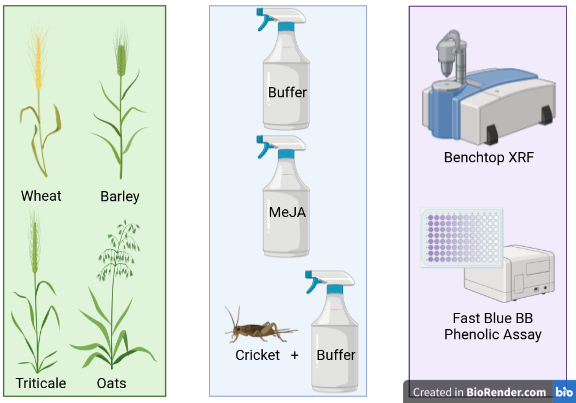
\includegraphics[width = \textwidth]{images/Induction_schematic.png}
        \centering
        \caption{Experimental schematic for this study. We grew four species of cereal crops (left box) in a glasshouse. After 45 days, we applied one of three treatments to each plant, in a fully randomized manner (centre box). To analyse the response of leaf silicon and phenolic content, we used X-ray fluorescence (XRF) and the Fast Blue BB phenolic assay (right box).}
        \label{Fig:exp_design}
\end{figure}

\begin{figure}[h]
        \centering
        \begin{subfigure}[b]{0.49\textwidth}
                \centering
                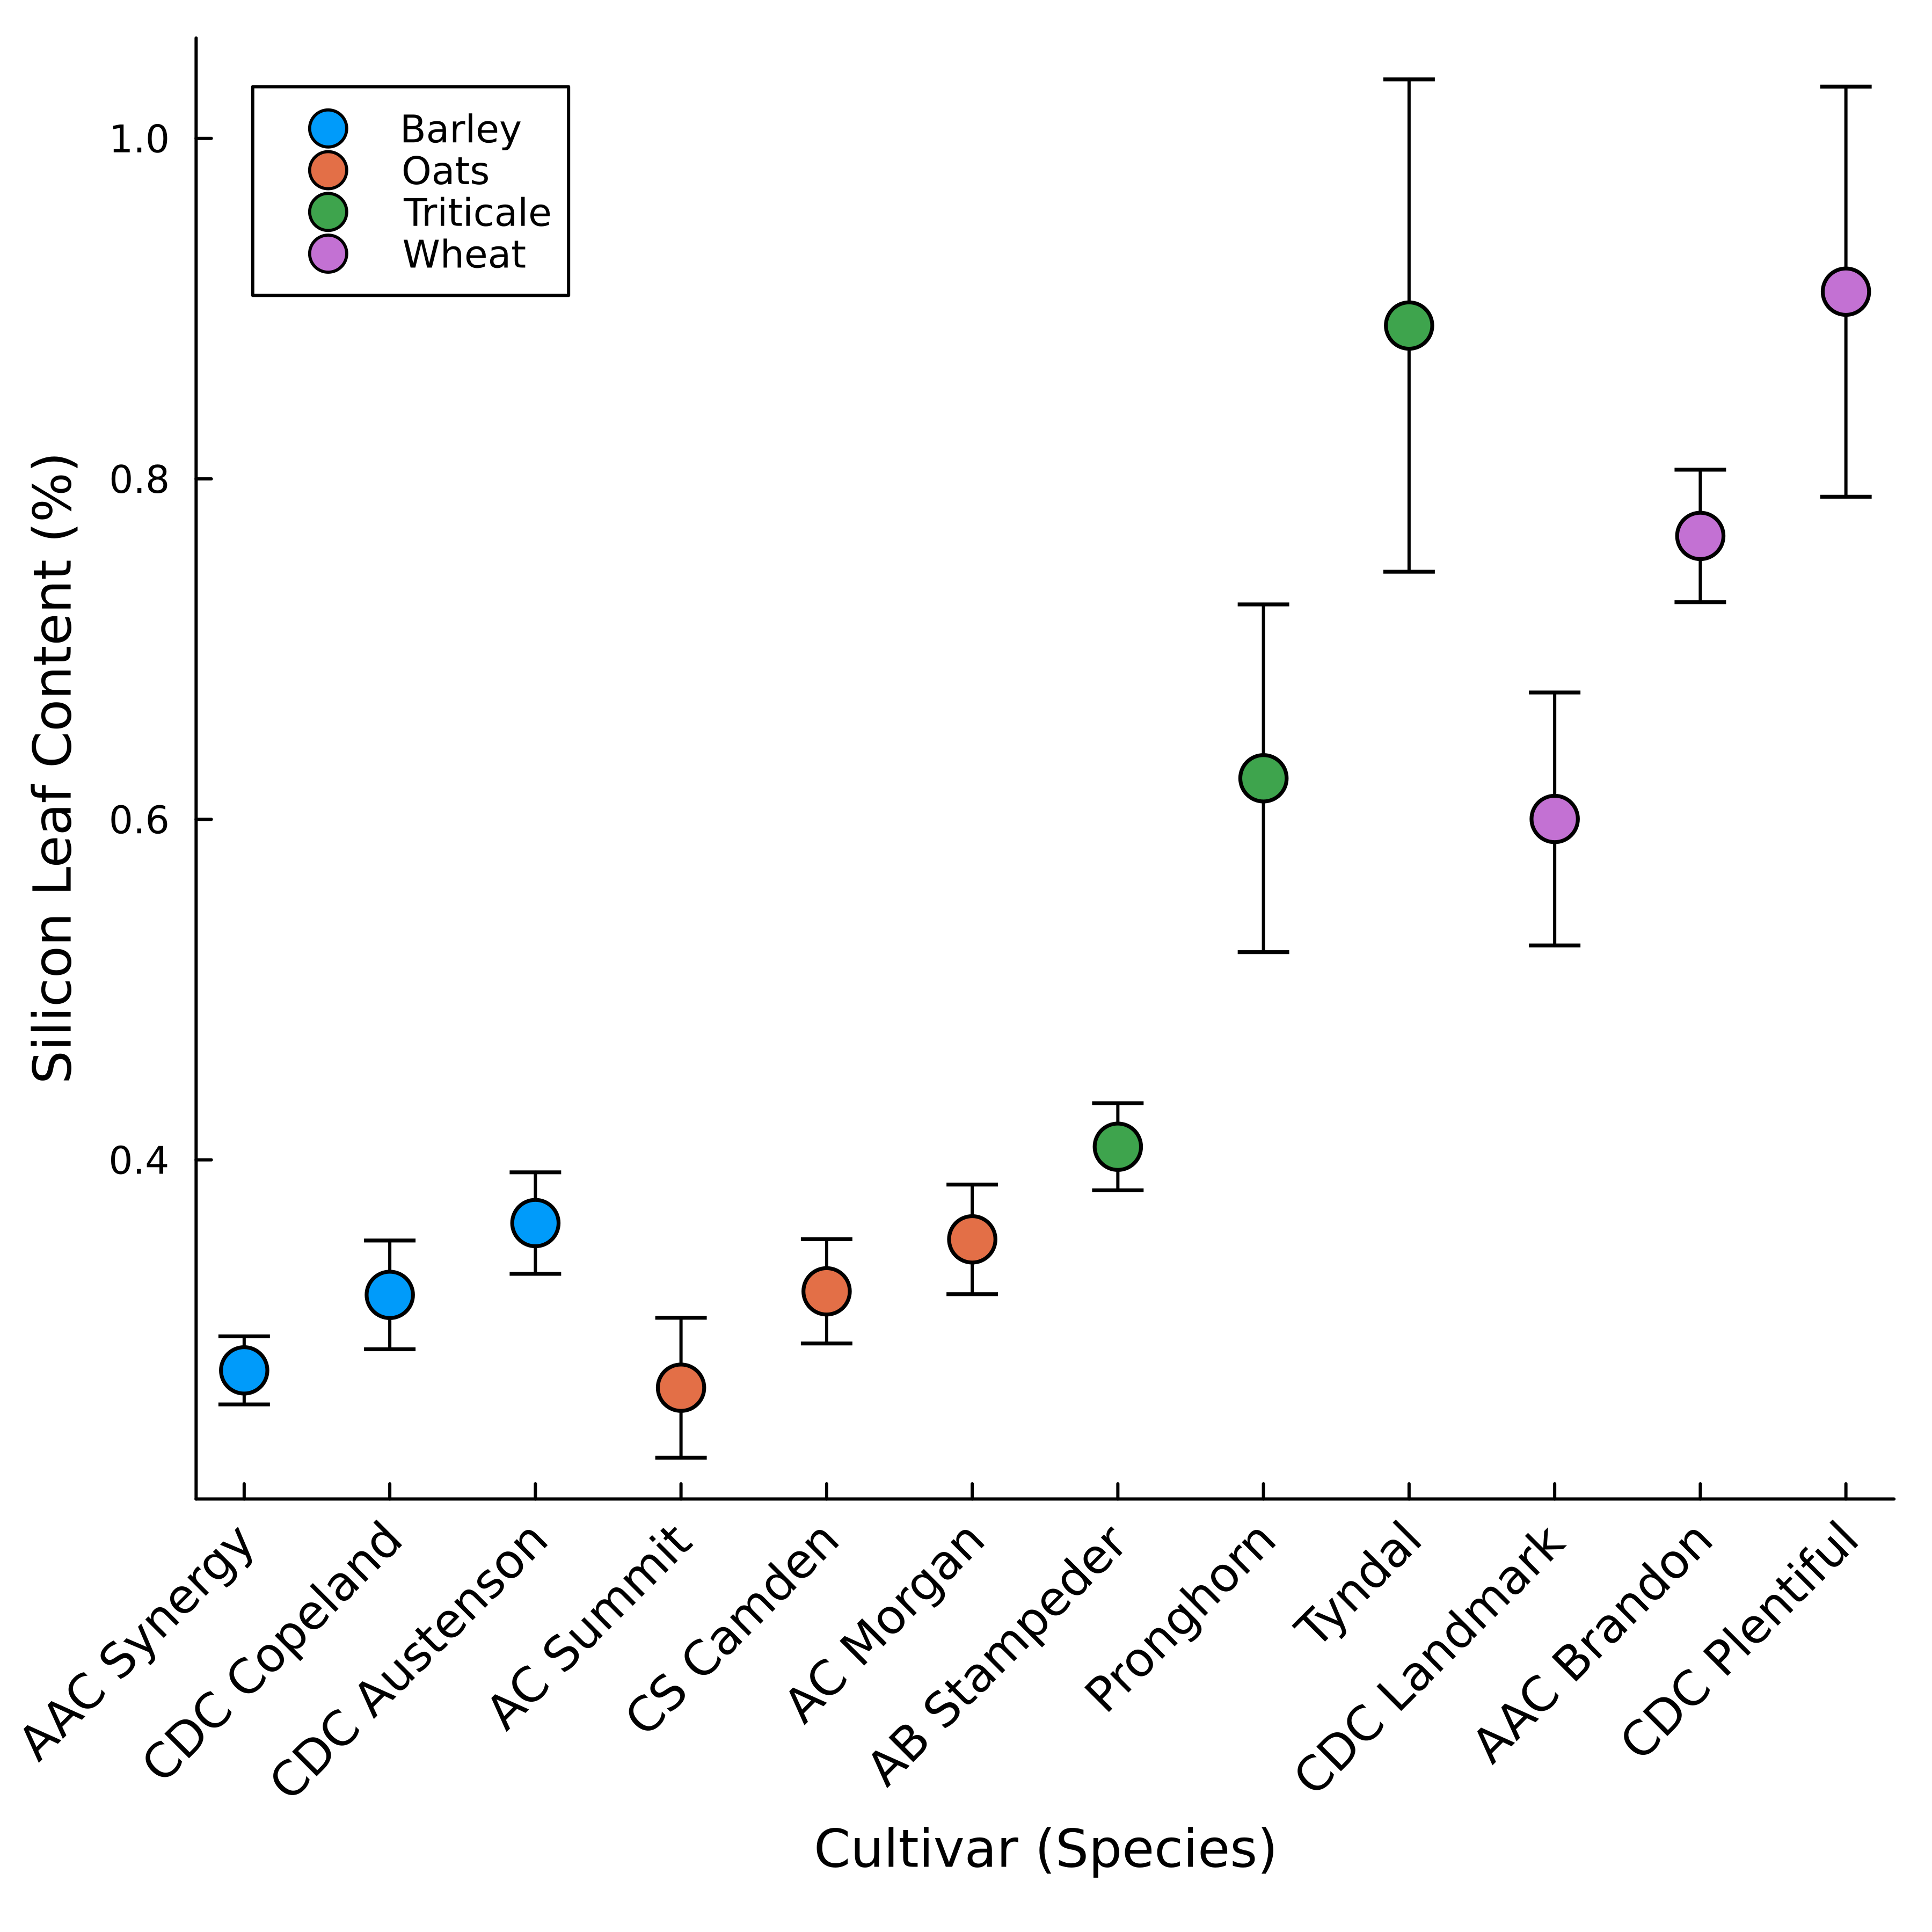
\includegraphics[width = \textwidth]{images/spp_si_content.png}
        \end{subfigure}
        \begin{subfigure}[b]{0.49\textwidth}
                \centering
                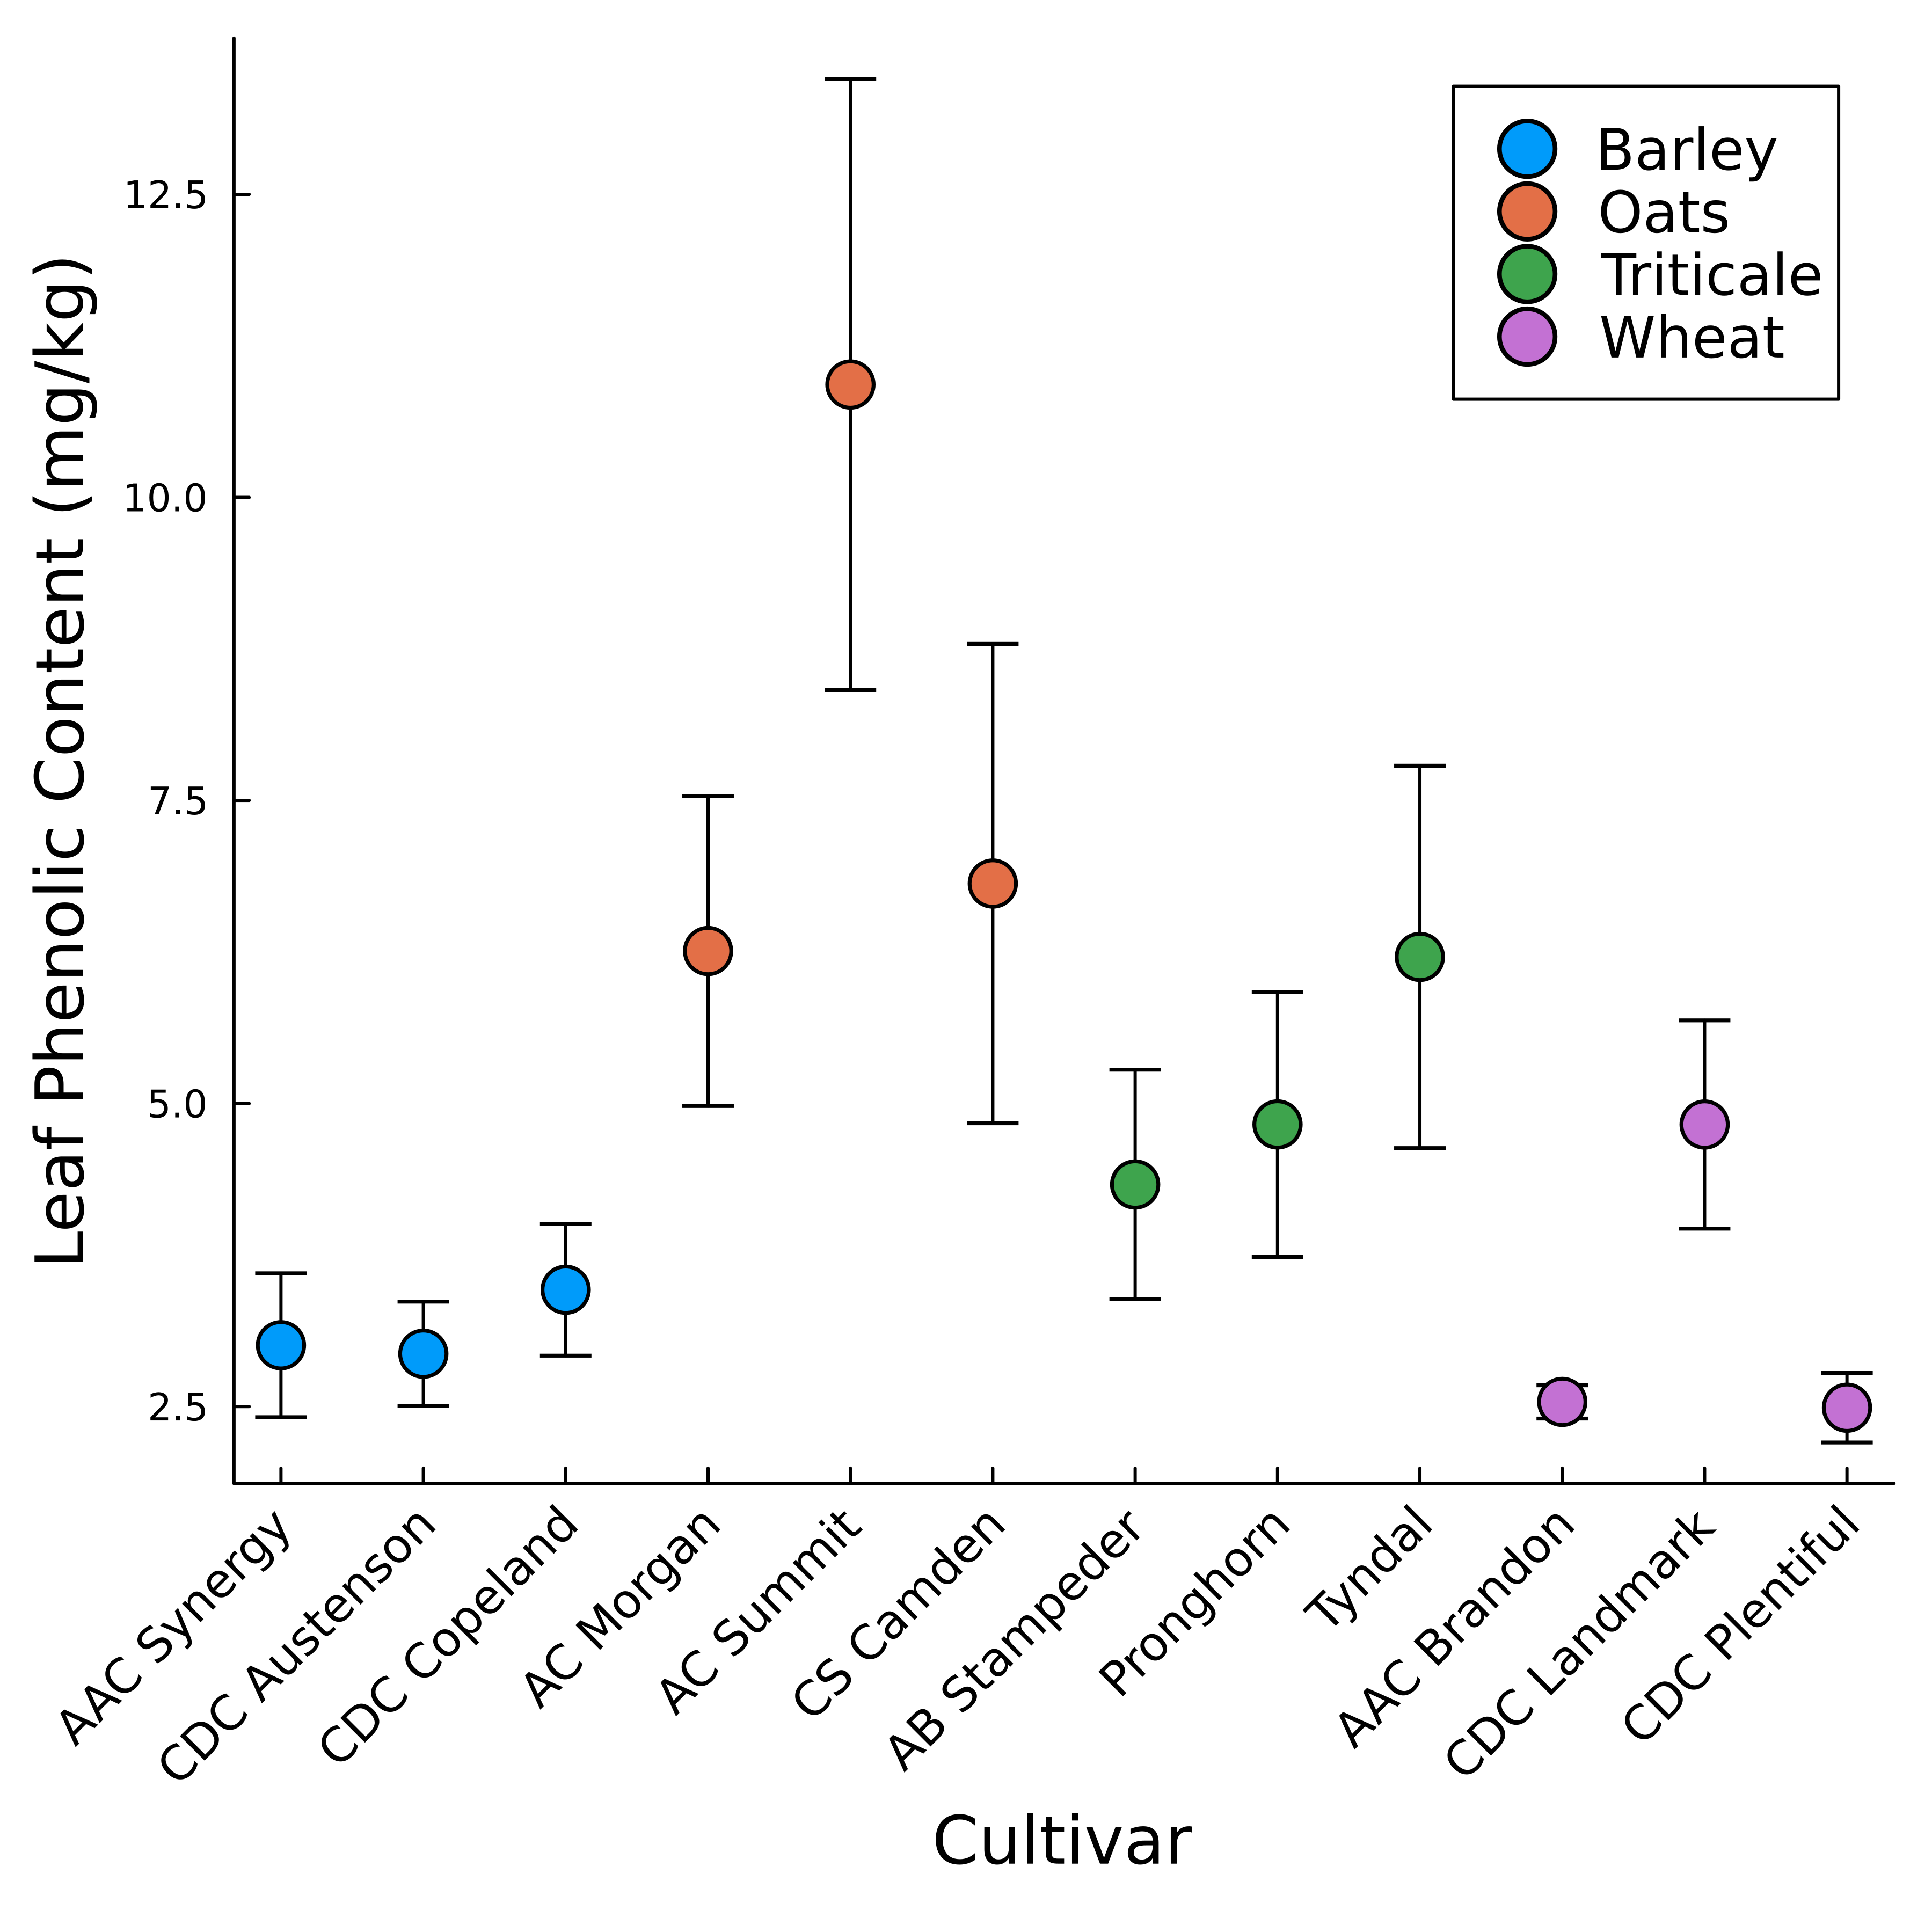
\includegraphics[width = \textwidth]{images/spp_phenolic_content.png}
        \end{subfigure}
                
        \centering
        \caption{Baseline (uninduced) silicon content (\% dry matter) and phenolic content (mg/kg) in the cereal cultivars used in this study. Cultivar species is indicated by point color. Error bars are 1 Standard Error.}
        \label{Fig:baseline_si}
\end{figure}

\begin{figure}[h]
        \centering
        \begin{subfigure}[b]{0.49\textwidth}
                \centering
                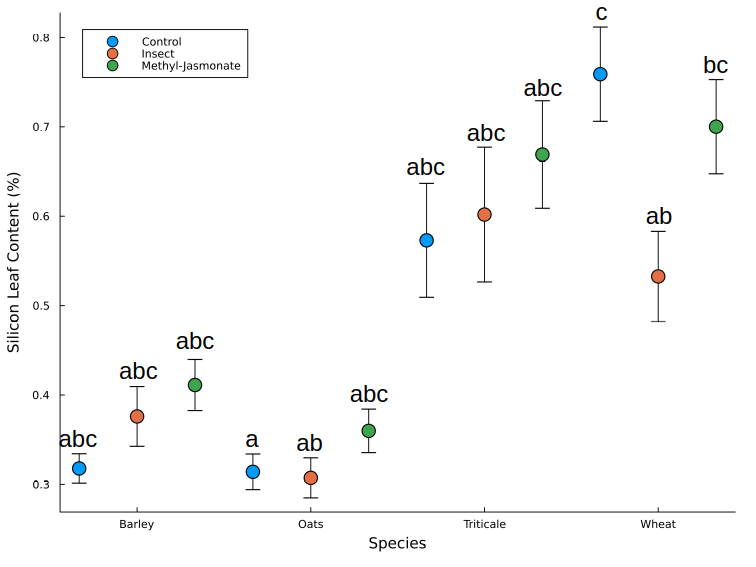
\includegraphics[width = \textwidth]{images/induction_plot_letters.png}
        \end{subfigure}
        \begin{subfigure}[b]{0.49\textwidth}
                \centering
                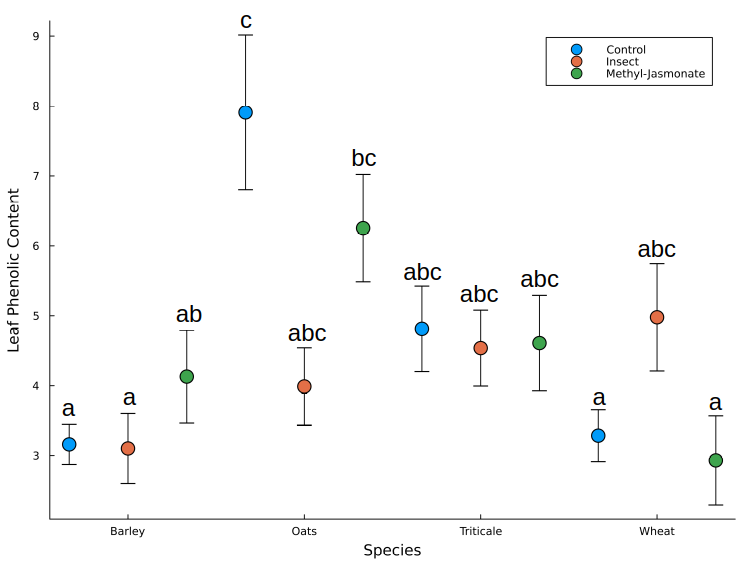
\includegraphics[width = \textwidth]{images/phenolic_induction_plot_letters.png}
        \end{subfigure}
        \caption{The response of leaf silicon content (left) and leaf phenolic content (right) for four cereal species across three defence induction treatments. We treated plants either with a 1mM methyl jasmonate spray, or exposure to house crickets (\textit{Acheta domesticus}). Leaves were sampled 18 hours after treatment, and were analysed for silicon using XRF or for phenolic content using the Fast Blue BB method. Dots and error bars are the mean $\pm$ 1 Standard Error.}
        \label{Fig:induction}
\end{figure}



\begin{figure}[h]
        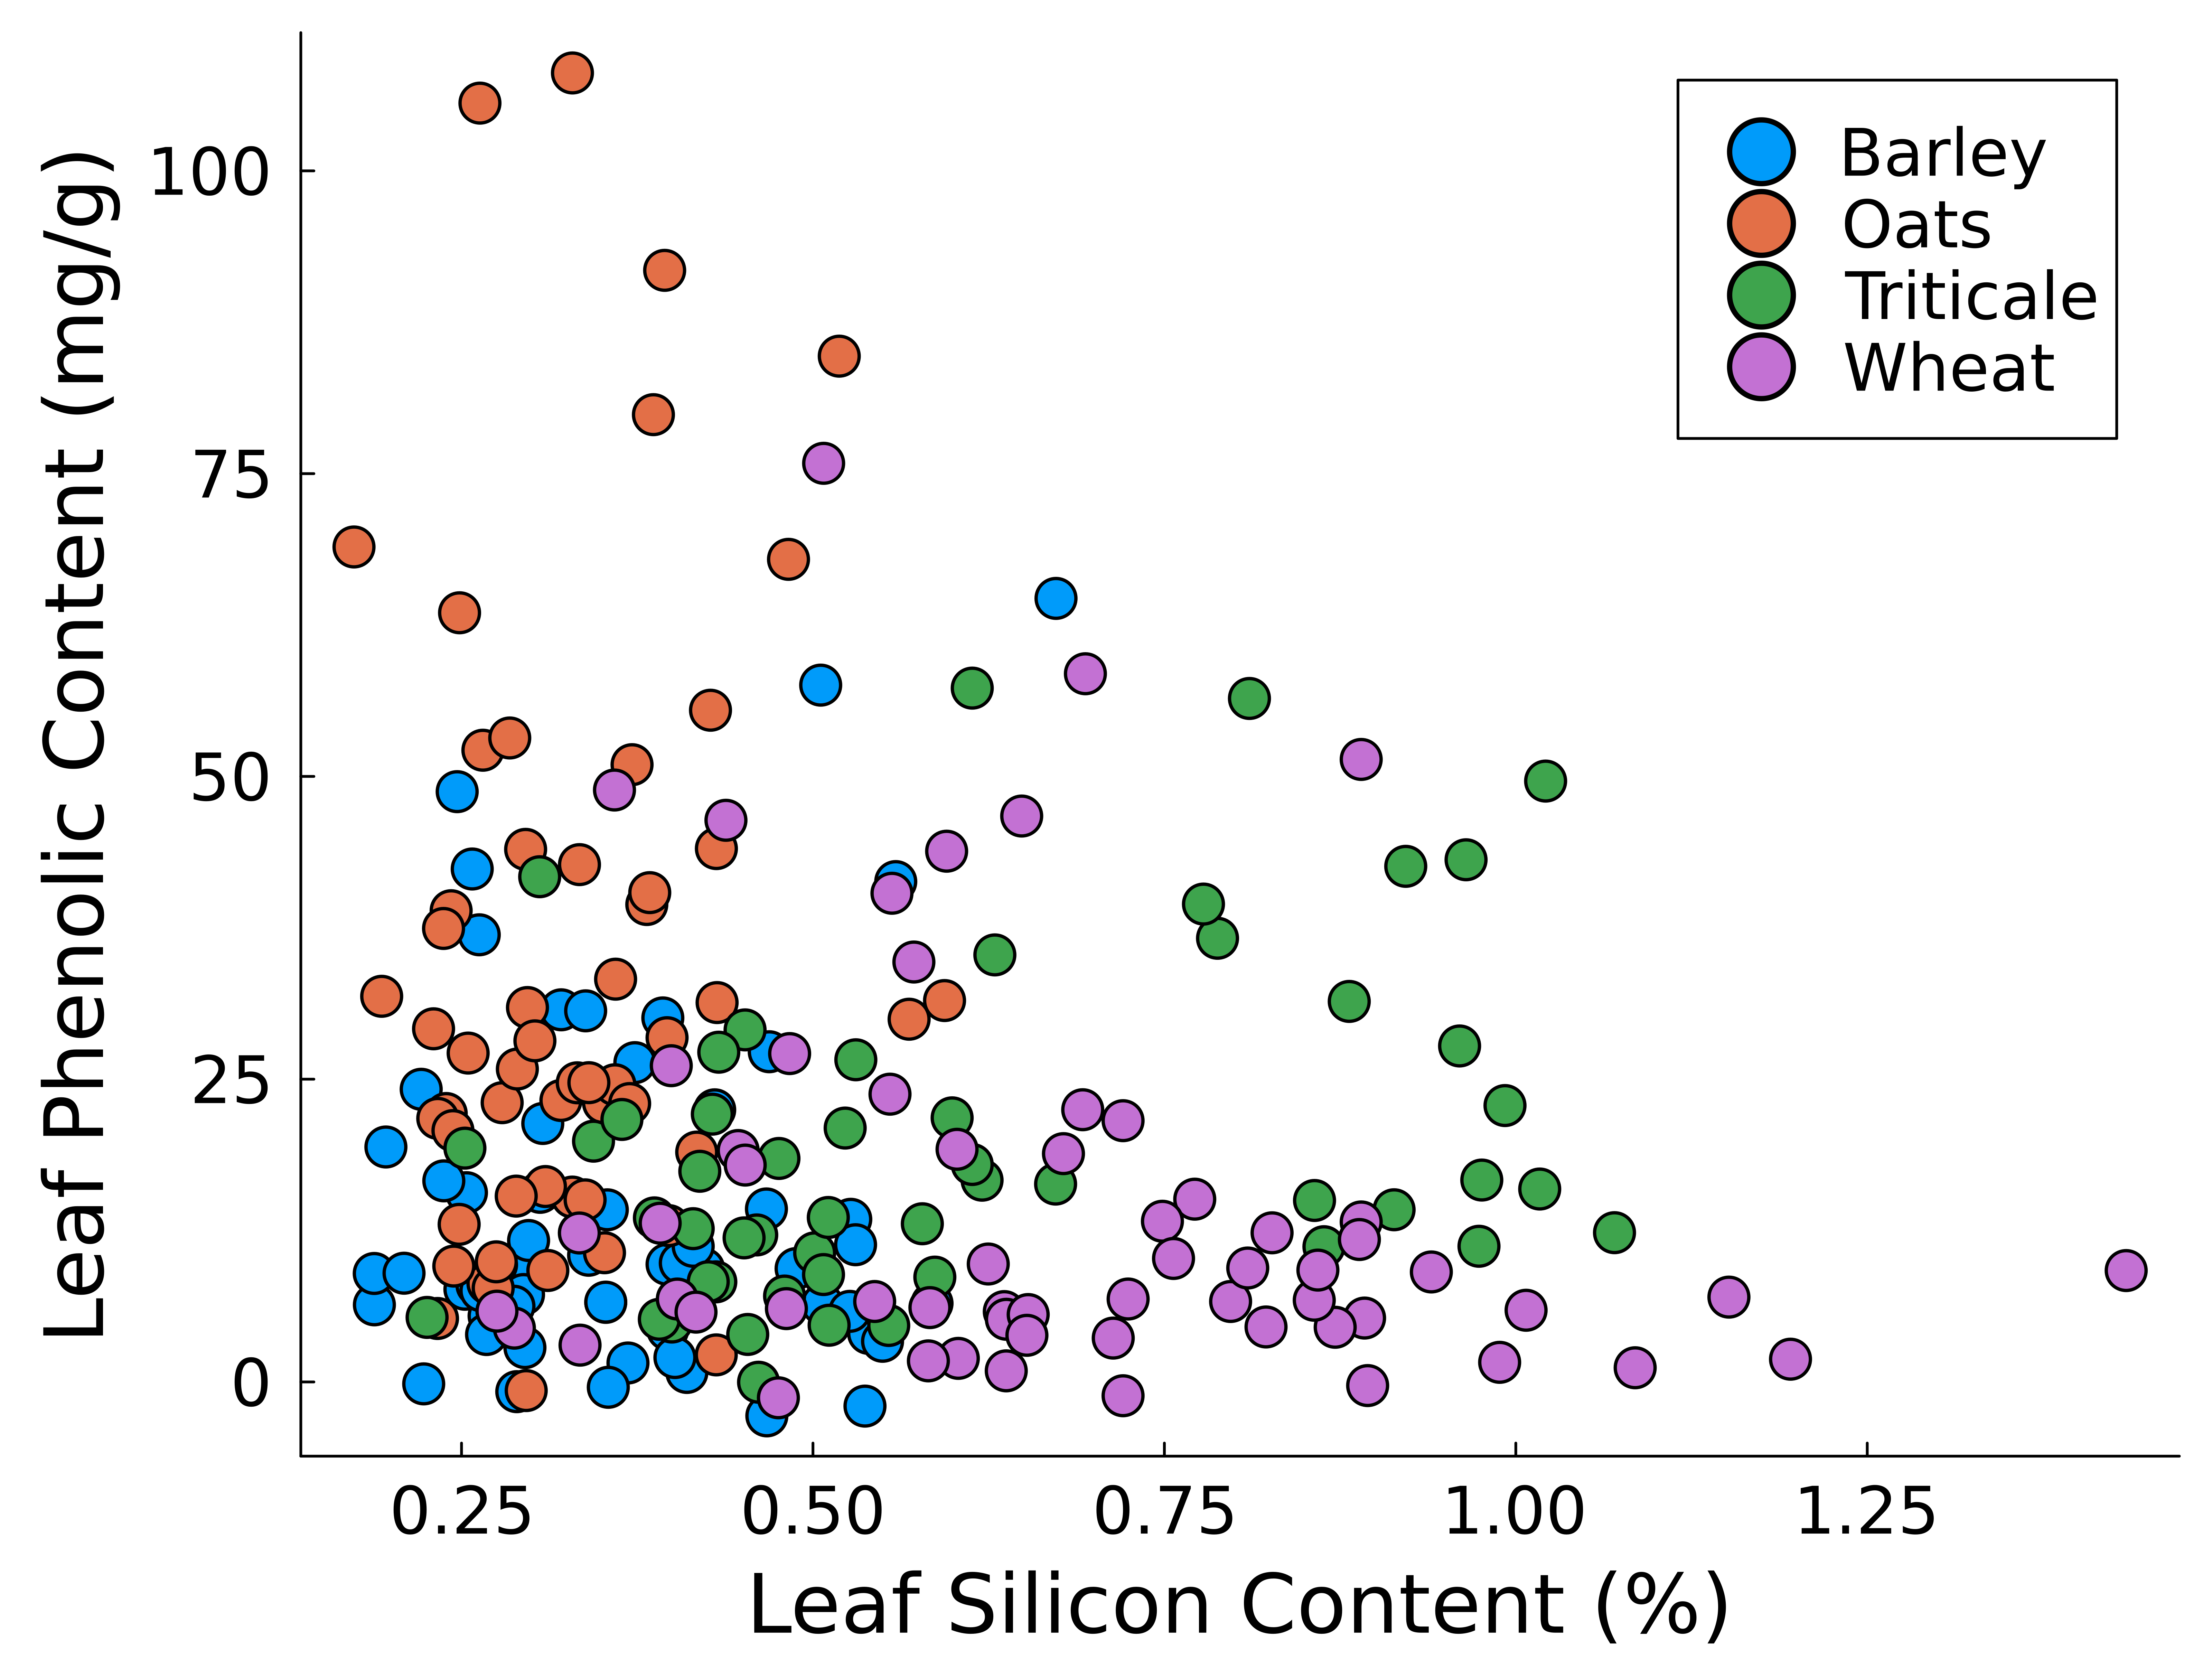
\includegraphics[width = \textwidth]{images/phenolic_silicon_regression.png}
        \centering
        \caption{The relationship between baseline (uninduced) silicon and phenolic content of leaves across four species of cereals. We measured leaf silicon content using XRF. We measured leaf phenolic content using the Fast Blue BB method.}
        \label{Fig:phe_si_scatter}
\end{figure}
\clearpage

\section{Supplementary Info}
\begin{landscape}
\begin{table}
        \centering
        \caption{Pedigrees of the cultivars used in this study}
        \begin{tabular}{ll>{\raggedright\arraybackslash}p{3cm}>{\raggedright\arraybackslash}p{3cm}>{\raggedright\arraybackslash}p{5cm}>{\raggedright\arraybackslash}p{4cm}}
          \toprule
          Species & Cultivar & Parent 1 & Parent 2 & Parent 1 Pedigree & Parent 2 Pedigree \\
          \midrule
          Barley & CDC Austenson & TR358 & 94Ab12271 & Not Available & Not Available \\
          Barley & AAC Synergy & TR02267 & Newdale & TR253/AC Metcalfe & CDC Stratus//TR236/WM862-6 \\
          Barley & CDC Copeland & WM861-5 & TR118 & Harrington & \\
          Oats & AC Morgan & OT526 & OT763 & 17578/Alfred & Fidler/Cascade \\
          Oats & Camden & SW Betania & Dominik & SW 151-7-95/SW 52-95 & Not Available \\
          Oats & AC Summit & Ronald & OT299 & W89329/AC Medallion & AC Rebel/Dumont 48 \\
          Triticale & Bunker & 95P105 & 85L0120006 & Pika-5/Yogui-1 & Spring triticale*n/RL4137 \\
          Triticale & Tyndal & Nimir-1/Hare-265//Erizo-9 & 88L012 & Nimir-1/Hare-265//Erizo-9 & Pronghorn*n/RL4137 \\
          Triticale & AB Stampeder & BULL 10/MANATI1//FARA S/CMH84.4414 & POLLMER 2.2.1 $\ast$2//FARA S/CMH84.4414 & BULL 10/MANATI1//FARA S/CMH84.4414 & POLLMER 2.2.1 $\ast$2//FARA S/CMH84.4414 \\
          Wheat & AAC Brandon & Superb/CDC Osler & ND744 & Superb/CDC Osler & ND2831/Parshall//ND706 \\
          Wheat & CDC Landmark & Unity & BW864 & McKenzie$\ast$3// BW174$\ast$2/Clark & YAQUI 50-ENANO/3$\ast$KALYANSONA \\
          Wheat & CDC Plentiful & BW282 & CDC Go & AC Elsa/AC Barrie & Grandin/SD3055 \\
          \bottomrule
        \end{tabular}
      \end{table}
      
      \end{landscape}

\clearpage



\chapter{Chapter 2: Genetic drivers of silicon accumulation in a wild ancestor of wheat}

\section{Introduction}

Over the past thirty years, plant silicon has emerged as an exciting possible tool to effect sustainable increases in crop production, with particular applicability in the cereal crops (\cite{reynolds_silicon_2016,christian_breeding_2022}). Cereal crops are globally important, covering over one-third of the world’s arable land, making up over 50\% of the daily caloric intake for most people (\cite{faostat, rudel_agricultural_2009, awika_major_2011}). Cereals are members of the grass family (Poaceae) and typically have relatively high plant silicon content ($\sim0.6 - 10\%$ total dry weight) (\cite{reynolds_silicon_2016}). Silicon's high abundance in many soils, high expression in cereal crops, and incredible broad spectrum effects on plant vigor and stress tolerance have made it a tantalizing target for improvements in agricultural yield and sustainability. 

Silicon underpins a variety of physiological and developmental strategies that plants use to cope with stress. Though plants can complete their life cycle in the absence of silicon, its influence on such a diverse range of plant physiological functions has caused researchers to emphasize its importance relative to other non-essential nutrients. For biotic stressors, silicon can reduce the damage plants experience from herbivory, increase resistance to fungal pathogens, and improve competitive ability with other organisms (\cite{fauteux_silicon_2005, katz_silicon_2019}). On the abiotic side, silicon supplementation improves plant resistance to soil salinity and heavy metal contamination, improves performance against temperature extremes and high irradiation, and helps plants to cope with drought stress (\cite{cooke_consistent_2016}). In comparing stressed plants grown in the absence or presence of silicon, silicon-exposed plants showed a transcriptome profile similar to unstressed plants (\cite{coskun_controversies_2019}). A current hypothesis explaining the broad-spectrum activity of silicon is presented in  \textcite{coskun_controversies_2019}. Their apoplastic barrier hypothesis suggests that silicon deposited in the apoplast of plant tissues modulates biological functions of the plant, and ecological interaction with natural enemies, yielding net positive increases in plant performance. Realizing these beneficial effects depends on the plant’s ability to efficiently source silicon from the soil and uptake it in sufficient amounts. Finding ways to improve crops towards increased silicon use efficiency is key to harnessing the benefits that plant silicon can confer. 

Plants gather silicon from the soil solution, using a suite of transporter proteins to pump it into their vascular systems and then transport it throughout the body (\cite{reynolds_silicon_2016}).  Variation in the relative expression of these transporters, as well as differences in the development of the end points for silicon deposition (silica cells), may drive phenotypic variation among individuals. Additionally, individuals may vary in their ability to scavenge silicon from the soil. The soluble form of silicon, silicic acid (SiOH4) has a maximum solubility in water of around 2 mM, though typical soil concentrations range from 0.1 mM to 0.6 mM (\cite{epstein_anomaly_1994}). Soluble silicon in the soil is derived primarily from the weathering of silicate minerals, and secondarily from the remobilisation of silicon in decaying plant material (\cite{de_tombeur_silicon_2021-1}). Weathering of silicates releases a host of plant nutrients including aluminium, silicon, iron, and phosphorus (\cite{de_tombeur_silicon_2021-1}). Soil biota can drive weathering, using organic acids and other molecules to complex metal ions off of soil aggregates, making them available for uptake by organisms (\cite{de_tombeur_silicon_2021}). Plant roots can release carboxylates and phytosiderophores to weather phosphorus and silicon out of soil minerals (\cite{de_tombeur_silicon_2021-1}). Along with Si and P mobilisation, manganese is often released, and taken up by plants roots. Previous research has used leaf manganese content to proxy for the carboxylate releasing activity of plants (\cite{lambers_leaf_2015}), yet so far we are unaware of any studies looking for quantitative variation among genotypes of leaf manganese. If we could identify regions of the plant genome associated with variation in leaf manganese content, we could follow up with more targetted studies looking for genes that influence root carboxylate release. This trait could eventually be incorporated into breeding programs, improving nutrient use efficiency, ultimately easing our dependence on external inputs to agricultural fields. 

The use of x-ray fluorescence (XRF) to quantify plant silicon has greatly reduced the costs, danger, and processing time of for studies focussing on this topic (\cite{reidinger_rapid_2012}). XRF works by using low-power x-rays to excite elements in the sample, and measures the resulting emitted light. One of the most exciting features of XRF is the fact that it can analyse multiple elements at once, allowing for broad characterisation of the sample for most elements heavier than aluminum. Though XRF is an established technique to measure plant silicon, its may also be used to measure other metals of interest, including manganese. In this study we use XRF to quantify variation in silicon and manganese content among a diversity panel of a wild ancestor of bread wheat, \textit{Aegilops tauschii}. This panel has publicly available sequence data \cite{gaurav_population_2022}, allowing us to perform a genome-wide association study to link silicon and manganese variation to genotypic variation, laying the groundwork for future, more targetted explorations of the genome. Identifying genetic controls over these traits will hopefully help develop breeding targets to improve plant performance and safeguard yeilds against a destabilizing climate.

\section{Methods}

\subsection{Plant growing conditions}

For this experiment, we used the L2 panel of Aegilops tauschii from \textcite{gaurav_population_2022}. This panel is a 151 genotype subset of the full \textit{Aegilops tauschii} panel, selected for high diversity in nucleotide-binding leucine rich repeats receptor (NLR) genes. We grew the L2 panel at three different sites; two of the sites were outdoors on the University of British Columbia campus, with planting occurring in the fall, while the third site was a glasshouse, where we vernalised seedlings in growth chambers prior to transplanting into pots. For full site details see Supplementary Table S1. Using 151 accessions, we started trays of seedlings in glasshouse or growth chamber environments. At approximately eight weeks after germination, seedlings were transplanted to their field sites. For each environment, we started four replicates of each accession. We planted the plants in a randomized block design, to minimize the effects of soil heterogeneity on our phenotype measurements. Each outdoor block was a 16 m\textsuperscript{2} square, with plants arranged $\sim$35 cm apart. Shortly after transplanting to the field sites, we applied water-soluble fertilizer to improve transplant survival, as well as slow-release fertilizer pellets. Field transplantation took place on the 15th of October 2021 and the 16th of December 2021. For the glasshouse environment, we started seedlings in growth chambers in January 2022. After 12 weeks, we moved the seedlings to vernalisation chambers (4ºC, 8:16h light:dark) for eight weeks. We then transplanted these plants into 10cm square pots filled with SunGro potting mix and amended with 0.17g of silicic acid (Tixosil 68B, Solvay). Pots were arranged using the same randomized block design, adapted to fit on two flood tables. To ensure a comparable life stage across environments at time of harvest, these plants grew for three months (mid June – mid September 2022), until they had mature flower heads. 

\subsection{Plant harvest and sample preparation}

  

\subsection{Sample analysis}

To analyse the silicon and manganese content of the accessions, we followed the XRF procedure presented in \textcite{reidinger_rapid_2012}. In short, we pressed leaf powder into 13mm diameter pellets at 300 bar of pressure and analysed the resulting pellets in an Olympus Vanta p-XRF device mounted in a bench stand. For beam 1 (manganese), we used a 20 second read time, while for beam 2 (Si), we used a 45 second read time. Based on preliminary trials, we determined these times to be a suitable trade-off between throughput and accuracy. For each pellet, we took two technical replicates, scanning each side of the pellet once. To minimize cross-contamination between samples, we cleaned the pellet press and XRF device after each sample. We calibrated our measurements against a standard curve of methyl-cellulose spiked with silicic acid, as well as certified reference materials (WEPAL-IPE-151, WEPAL-IPE-152).

\subsection{Statistical analysis}

To visualize the variability of silicon and manganese content within genotypes across environments, we converted elemental content into a rank, averaged ranks across environments, and plotted (Figure \ref{Fig:rank_plots}). 
To look for evidence of root exudation associated with silicon content, we tested a correlation between observed leaf silicon and manganese content. Prior to the analysis, we plotted histograms of silicon and manganese concentrations. We observed right-skew for both elements and applied a log-transformation. To control for intersite-variation we further transformed our measurements from log(concentration) to site-specific standard scores ($\frac{X - \mu}{\sigma}$). We then used the \verb|lmerTest| and \verb|MuMIn| (\cite{kuznetsova_2017_lmerTest,barton_2023_mumin}) packages in R 4.2.2 (\cite{r_core_team_2022}) to regress leaf manganese content on leaf silicon content. We used a random effect of Genotype to control for genotype-specific differences in silicon content. We used the R package \verb|MuMIn| (\cite{barton_2023_mumin} to estimate the $R^2$ value of our mixed model.

To perform the GWA analysis, we followed the methodology and code published in \textcite{gaurav_population_2022}. For brevity, the methodology of this manuscript only describes the steps we took using the data generated from \textcite{gaurav_population_2022}. For full details on how they generated the sequence data and prepared the final data sets refer to their manuscript. As per \textcite{gaurav_population_2022}, to reduce the computational intensity of our analysis, we prefiltered the total $k$-mer matrix to remove $k$-mers with a low chance of being informative. For each environment, we ran the GWAS, filtered $k$-mers with an association score of $<6$, and plotted the remaining $k$-mers. We calculated our bonferroni correction threshold using the \verb|knum_bonf.py| script provided by \textcite{gaurav_population_2022}. For peaks that were significant in at least two environments, we cross-referenced the location with the Aet v5.0 assembly in NCBI (\cite{wang_aegilops_2021}), looking for annotated genes that matched our observed peak locations. 

\section{Results}

 Silicon content in \textit{Aegilops tauschii} ranged from 0.784\% to 11.473\%. There were notable differences in silicon content based on the growing environment. The glasshouse plants averaged $1.450\% \pm 0.032 (SE)$, while the two outdoor environments averaged 4.935\% $\pm$ 0.108 and 6.471\% $\pm$ 0.132. Manganese content varied from 36.5 ppm to 1296.5 ppm, and averaged $225.1 \pm 25.45$ ppm (SE) in the glasshouse environment, and $ 71.05 \pm 2.571 ppm (SE)$ and $ 224.0 \pm 11.01 (SE)$ for the two outdoor growing environments. The results summarized in our rank plots (Figure \ref{Fig:rank_plots}) show that there are weak g. Silicon and manganese showed significant positive correlation ($\beta = 0.278 \pm 0.051, z = 5.46, p<0.0001, R^2_{marginal} = 0.05, R^2_{conditional} = 0.35 $) (Figure \ref{Fig:mn_si_regression}). Overall, our analysis revealed no regions of the \textit{Aegilops tauschii} genome that have significant associations across environments with silicon content (Figure \ref{Fig:si_peak_plot}), nor with manganese content (Figure \ref{Fig:mn_peak_plot}). For manganese, we detected a number of peaks in each environment that exceeded the threshold for significance. However, when comparing across environments, we found no regions that consistently exceeded the threshold significance. We did however find 11 regions exceeding the significance threshold that were present in both of our growing environments with real soil, though absent in the glasshouse environment (Table \ref{tab:peaks_and_genes}). Of these genes, three had associated genes in NCBI. Two of the genes were uncharacterised non-coding RNA genes. The third gene codes for CASP-like protein 5B3. 

\section{Discussion}

We observed major differences in silicon and manganese content between our growth environments, and did not find consistent correlations between genetic variation and variation in silicon content. Our rank plots revealed that relative content of both silicon and manganese is not stable across environments. This suggests strong genotype by environment interactions, which likely reduced our ability to detect genetic contributions to the silicon and manganese phenotype. Interestingly, we detected a number of peaks for leaf manganese content, though many of these were only found in a single environment. Though we detected no peaks present in all three growing environments, we detected 11 regions that were significant in both outdoor environments. Compared to the glasshouse environment, the outdoor environments likely exposed the plants to a soil environment in which root exudation yeilds nutrients for uptake. Root exudation of organic acids and chelating agents liberates phosphates and silicates from inorganic pools (\cite{de_tombeur_silicon_2021-1,lambers_plant_2008}). In the glasshouse environment, we grew plants in standard potting mix, which is high in organic matter with a relatively low inorganic component. In this soil context, root exudation is unlikely to yield appreciable nutrient liberation. The high manganese content found in the glasshouse plants is most likely due to the watering regime they experienced. We watered these plants using municipal tap water. In the Vancouver region, this water is sourced from reservoirs in the surrounding mountains, which themselves are filled from ground runoff. Nearby groundwater wells have issues with high manganese content (\cite{hu_drinking_2020}). A constant supply of soluble manganese in the irrigation the glasshouse plants likely accounts for the elevated manganese content. 

Our observations of a correlation between silicon and manganese content could be evidence of root-exudate driven silicon uptake. It is possible that this positive correlation is due to a nutrient effect more generally, where manganese and silicon covary in availability in the soil. However, further regressions show that silicon only shows positive correlations with iron and manganese, both of which are mobilized by root exudation (Supplementary Fig [Number]) (\cite{de_tombeur_silicon_2021-1}). Unfortunately, only one MTA is located in a coding-region of the genome. LOC109751197 codes for a CASP-like protein, involved in the casparian strip. The presence of a SNP in this region is negatively correlated with manganese content. CASP-like proteins are involved in cell membrane modification, and can form transmembrane scaffolds (\cite{roppolo_functional_2014}). This leads to a puzzling interpretation, where defects in a gene involved membrane modification (likely reducing permeability) decrease manganese uptake.  The uncharacterized nature of the gene in question makes more indepth interpretation of the results difficult, but provides a target for future investigations into genomic controls over manganese uptake.

Silicon interacts with manganese in the leaf, binding manganese to the cell wall and reducing manganese concentrations in the cell symplast (\cite{rogalla_role_2002}). Root exudation is most important under limited nutrients, and silicon-exudate dynamics have been best characterized in well-weathered soils (\cite{lambers_plant_2008,de_tombeur_shift_2021,de_tombeur_silicon_2021-1}). In agricultural soils, it is unlikely that plants would be exposed to such nutrient poor conditions, and so the specific dynamics of root exudation and silicon mobilisation deserve further investigation. Root exudation also results in increased soil carbon content, and there is interest in implementing cropping and fertilisation systems with an explicit focus on improving soil carbon through root exudation (\cite{cornelis_soil_2022}). In this context, understanding how increased root exudation may impact both silicon and metal uptake in plants is crucial, and future studies should pursue similar genetic approaches under limited phosphorus regimes to try and detect genes associated with root exudation activity. 

Depsite our inability to detect QTLs that reliably influence silicon or manganese content, this field of study still holds immense promise. We implemented a study design that we hoped would allow generalisations about the genetic regions we hoped to find. However, the use of multiple environments may have obscured QTLs that we may have otherwise detected in a single environment. The use of the diversity panel allowed for a rapid and low-cost initial search for loci asscociated with silicon and manganese content, but may have also limited our power to detect loci. The panel we used was a subset of the larger \textit{Aegilops tauschii} panel, and ours was selected specifically for diversity in disease-resistance genes. Utilizing the full panel of 384 genotypes could improve power of future studies. Alternatively, future researchers could attempt to create a mapping population. By using the silicon and manganese content rankings generated by this study, one could create a cross of a low and high genotype and use a traditional QTL mapping approach with the recombinant population. This approach might allow for more sensitivity in the analysis by reducing the overall genetic variation between genotypes in population, highlighting the genetically driven variation in silicon content.
\section{Acknowledgements}

\section{Data Availability}

\printbibliography

\section{Tables and Figures}

\begin{table}[ht]
        \centering
        \caption{Genomic regions with significant correlation to leaf manganese content, and the corresponding genes in the \textit{Aegilops tauschii} Aet v5.0 assembly. The assembly was scanned using the NCBI genome viewer tool.}
        \label{tab:peaks_and_genes}
        \begin{tabular}{lrrr}
        \hline
        \textbf{Chromosome} & \textbf{Peak Location} & \textbf{Range} & \textbf{Gene Symbol} \\
        \hline
        1D         & 201950k-201960k   & No Gene Found          &                 \\
        1D         & 402540k-402550k   & 402549667-402554765    & LOC109755172    \\
        1D         & 402540k-402550k   & 402547029-402549598    & LOC120968250    \\
        1D         & 418870k-418880k   & No Gene Found          &                 \\
        1D         & 418990k-419000k   & No Gene Found          &                 \\
        1D         & 419030k-419040k   & No Gene Found          &                 \\
        3D         & 575420k-575430k   & 575424894-575428979    & LOC109751197    \\
        4D         & 85300k-85310k     & No Gene Found          &                 \\
        4D         & 85310k-85320k     & No Gene Found          &                 \\
        4D         & 85330k-85340k     & No Gene Found          &                 \\
        \hline
        \end{tabular}
\end{table}
        

\begin{figure}[h]
        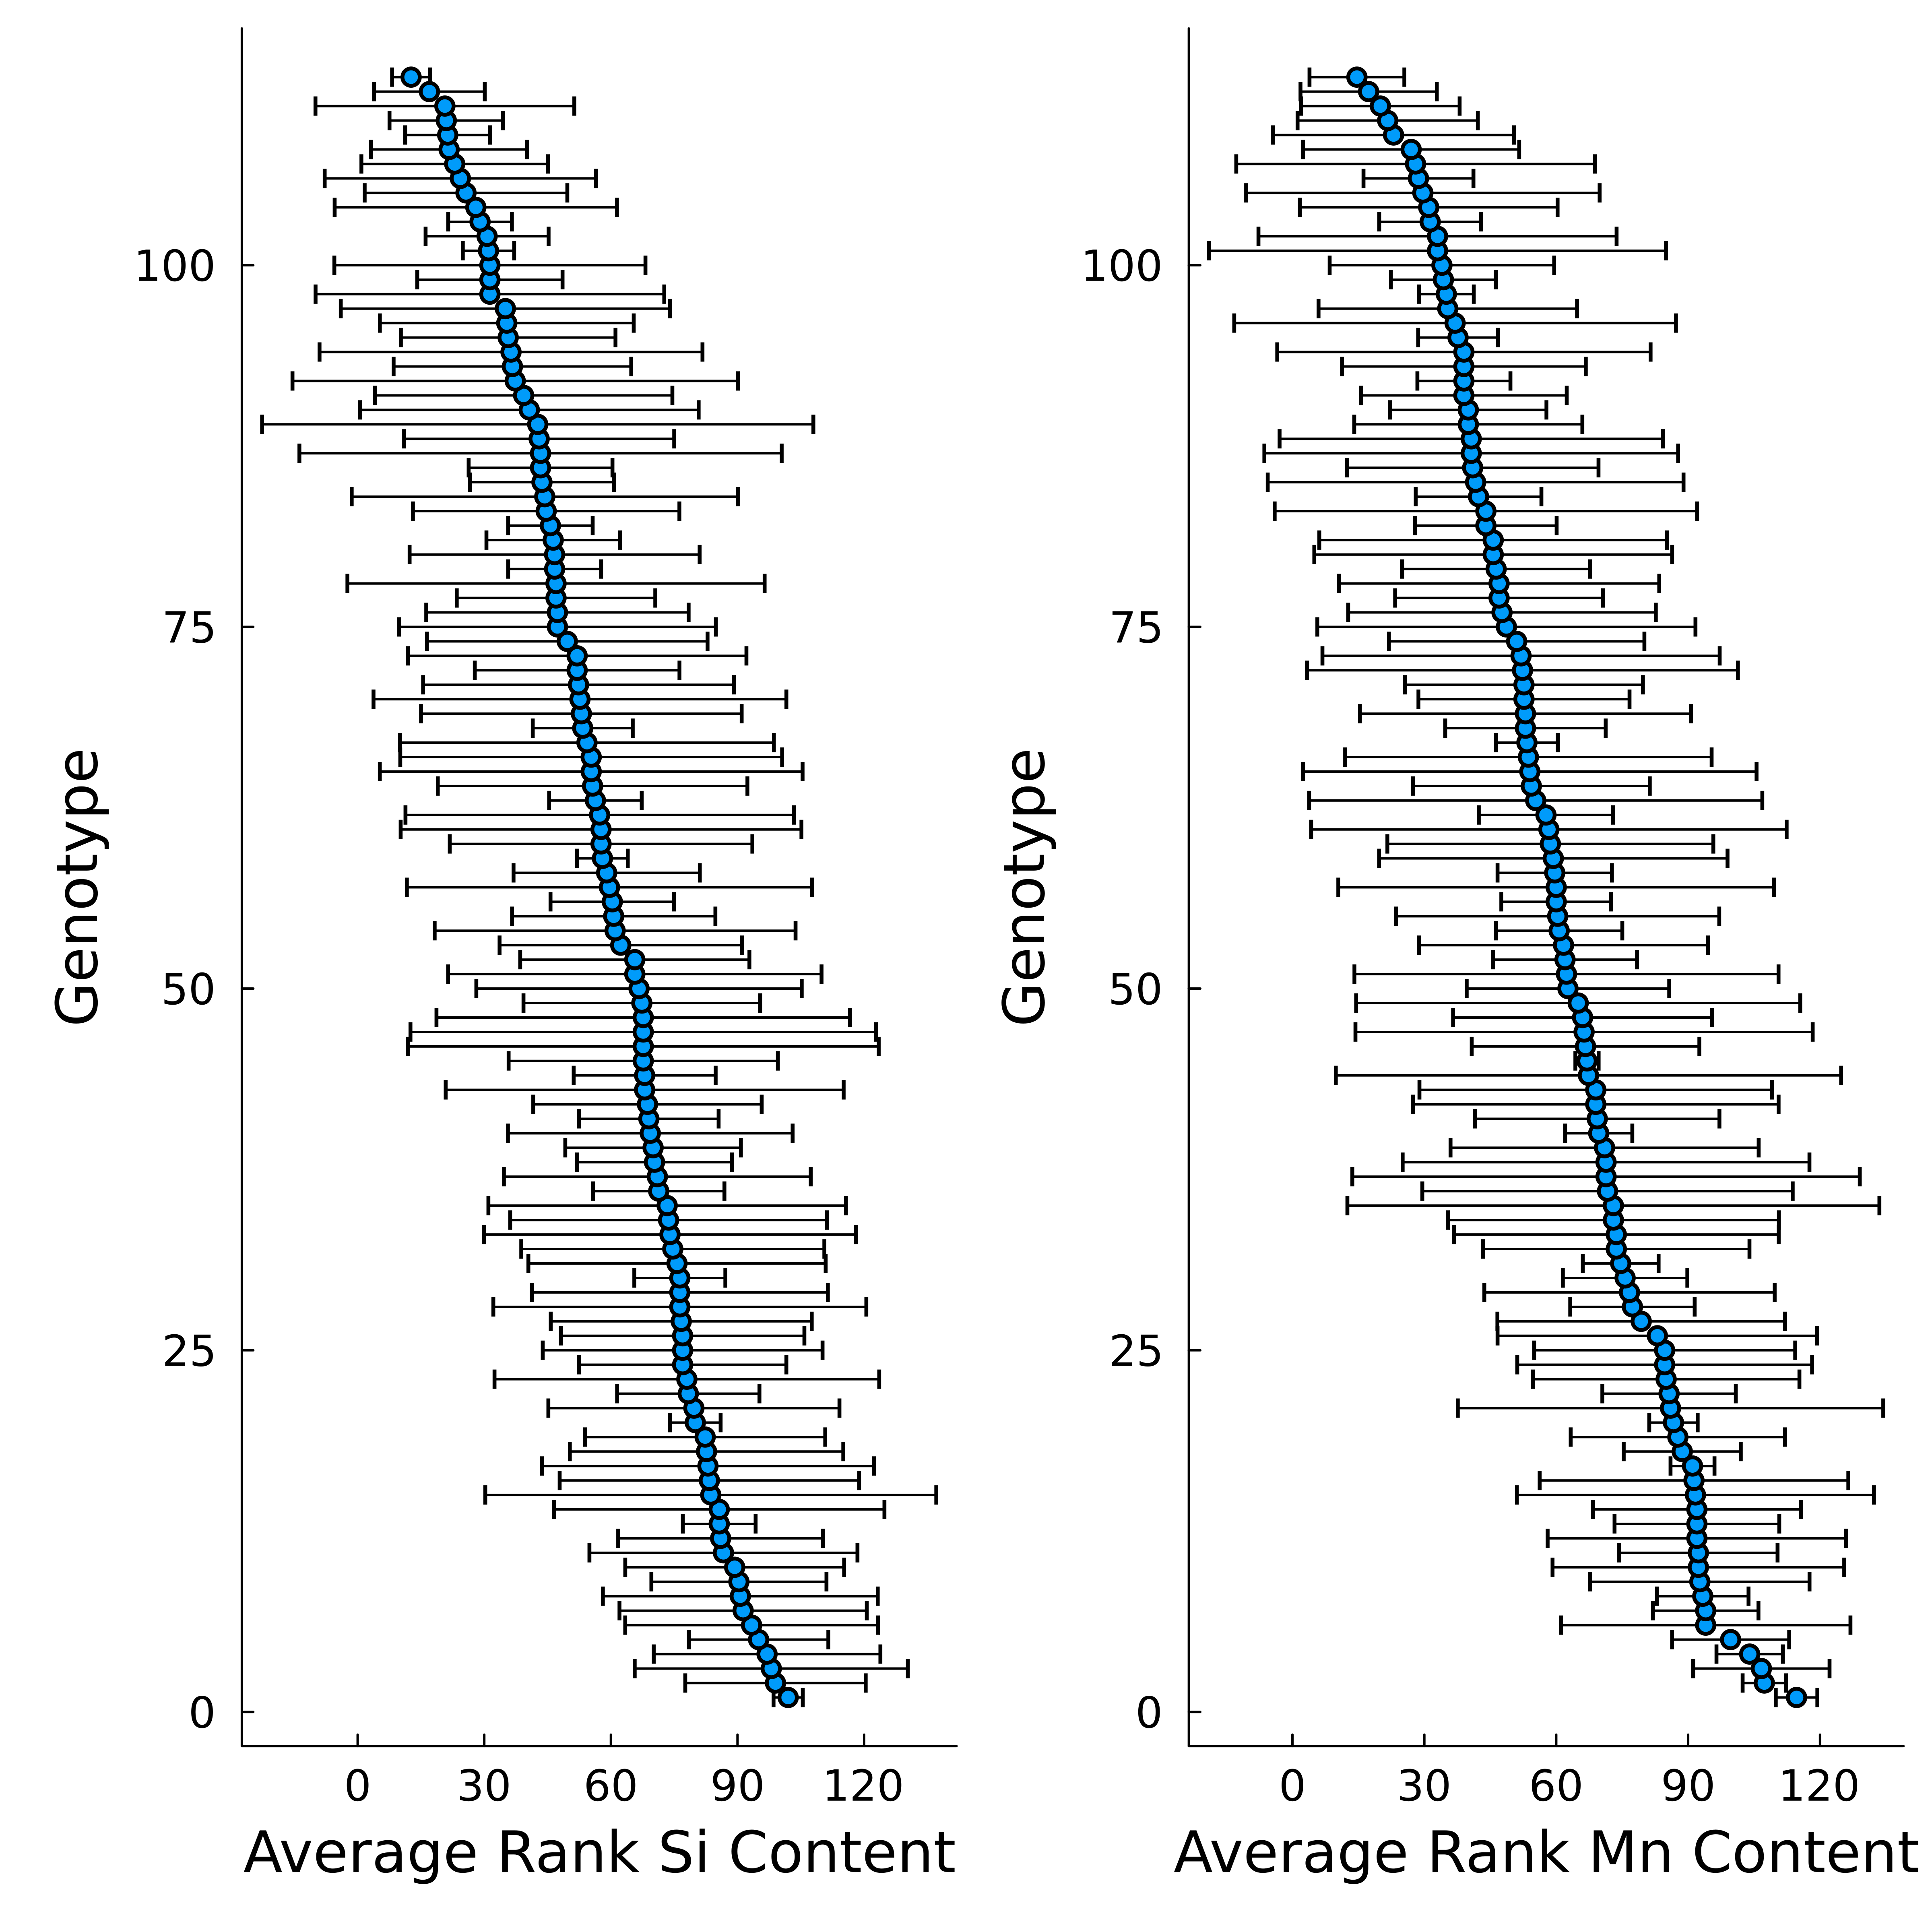
\includegraphics[scale=0.048]{images/rank_plots.png}
        \centering
        \caption{Average rank of silicon and manganese content of 113 genotypes of \textit{Aegilops tauschii} grown in three different environments. Error bars represent the standard deviation of rank.}
        \label{Fig:rank_plots}
\end{figure}

\begin{figure}[h]
        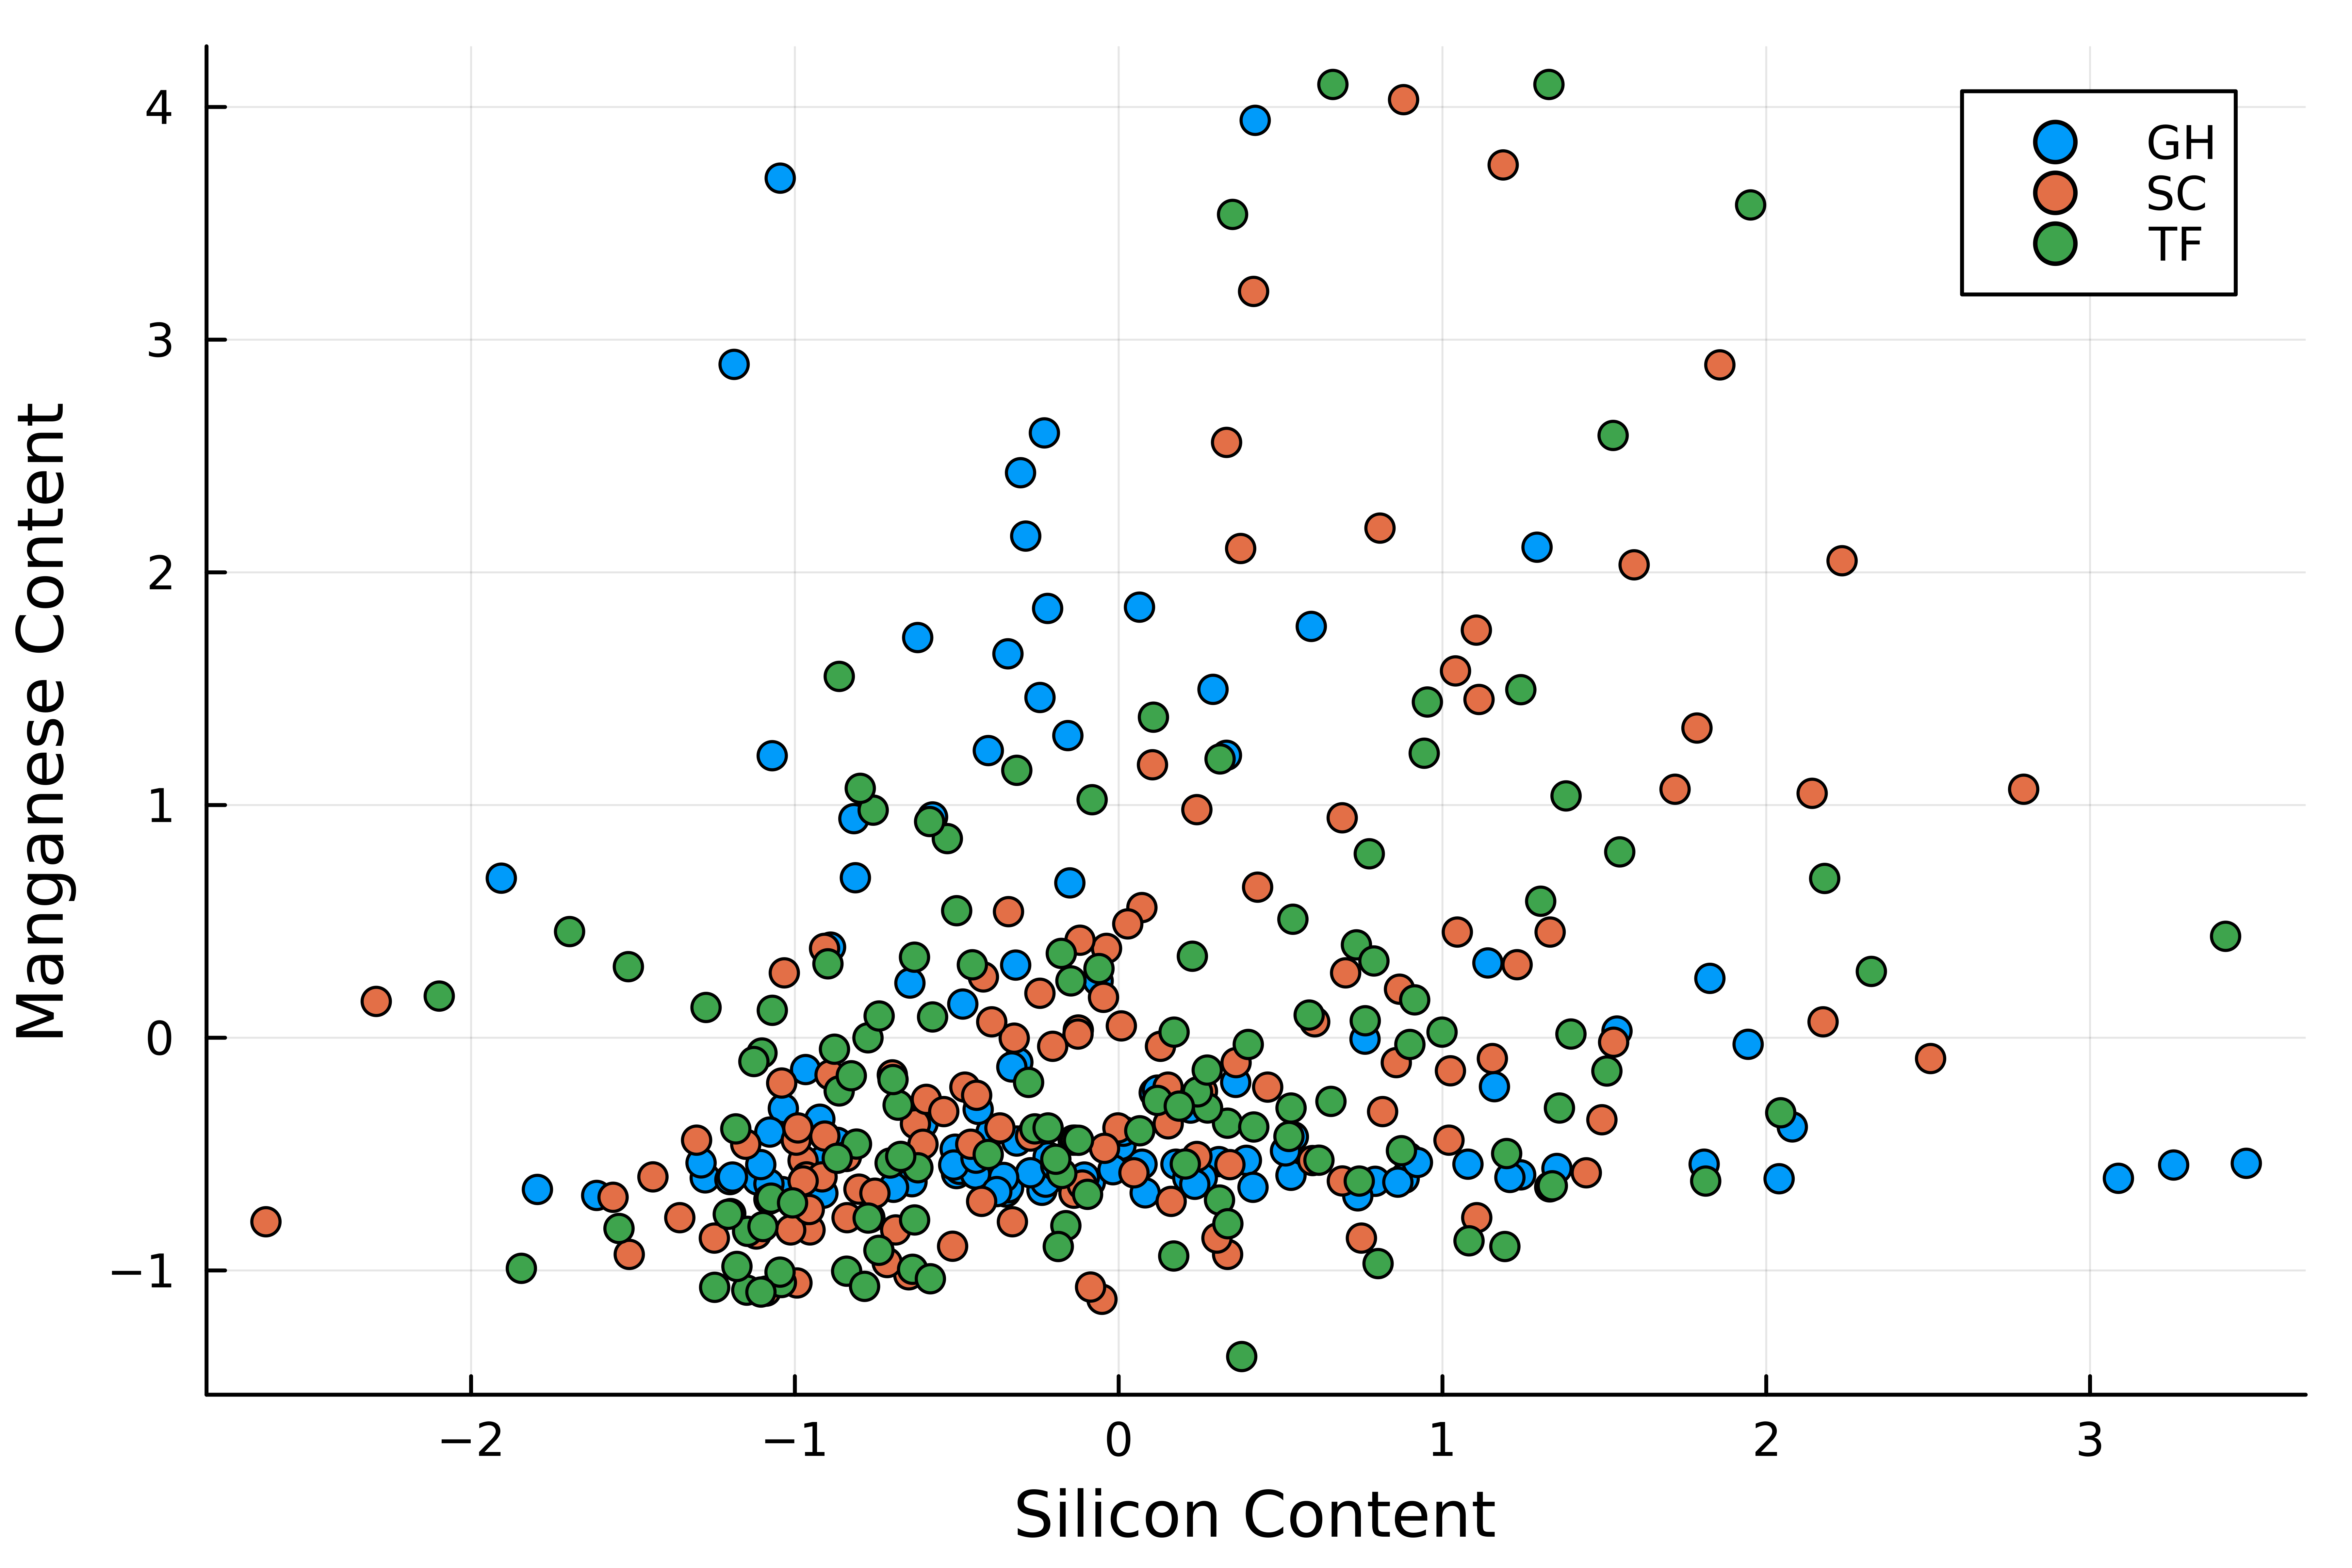
\includegraphics[scale=0.048]{images/si_mn_regression.png}
        \centering
        \caption{Scatter plot comparing leaf silicon and manganese content. Values for both elements were converted to standard scores to allow
        comparison between environments. Points are color coded according to environment. GH is the glasshouse environment, while SC and TF were two different outdoor plots.}
        \label{Fig:mn_si_regression}
\end{figure}

\begin{figure}[h]
        \centering
        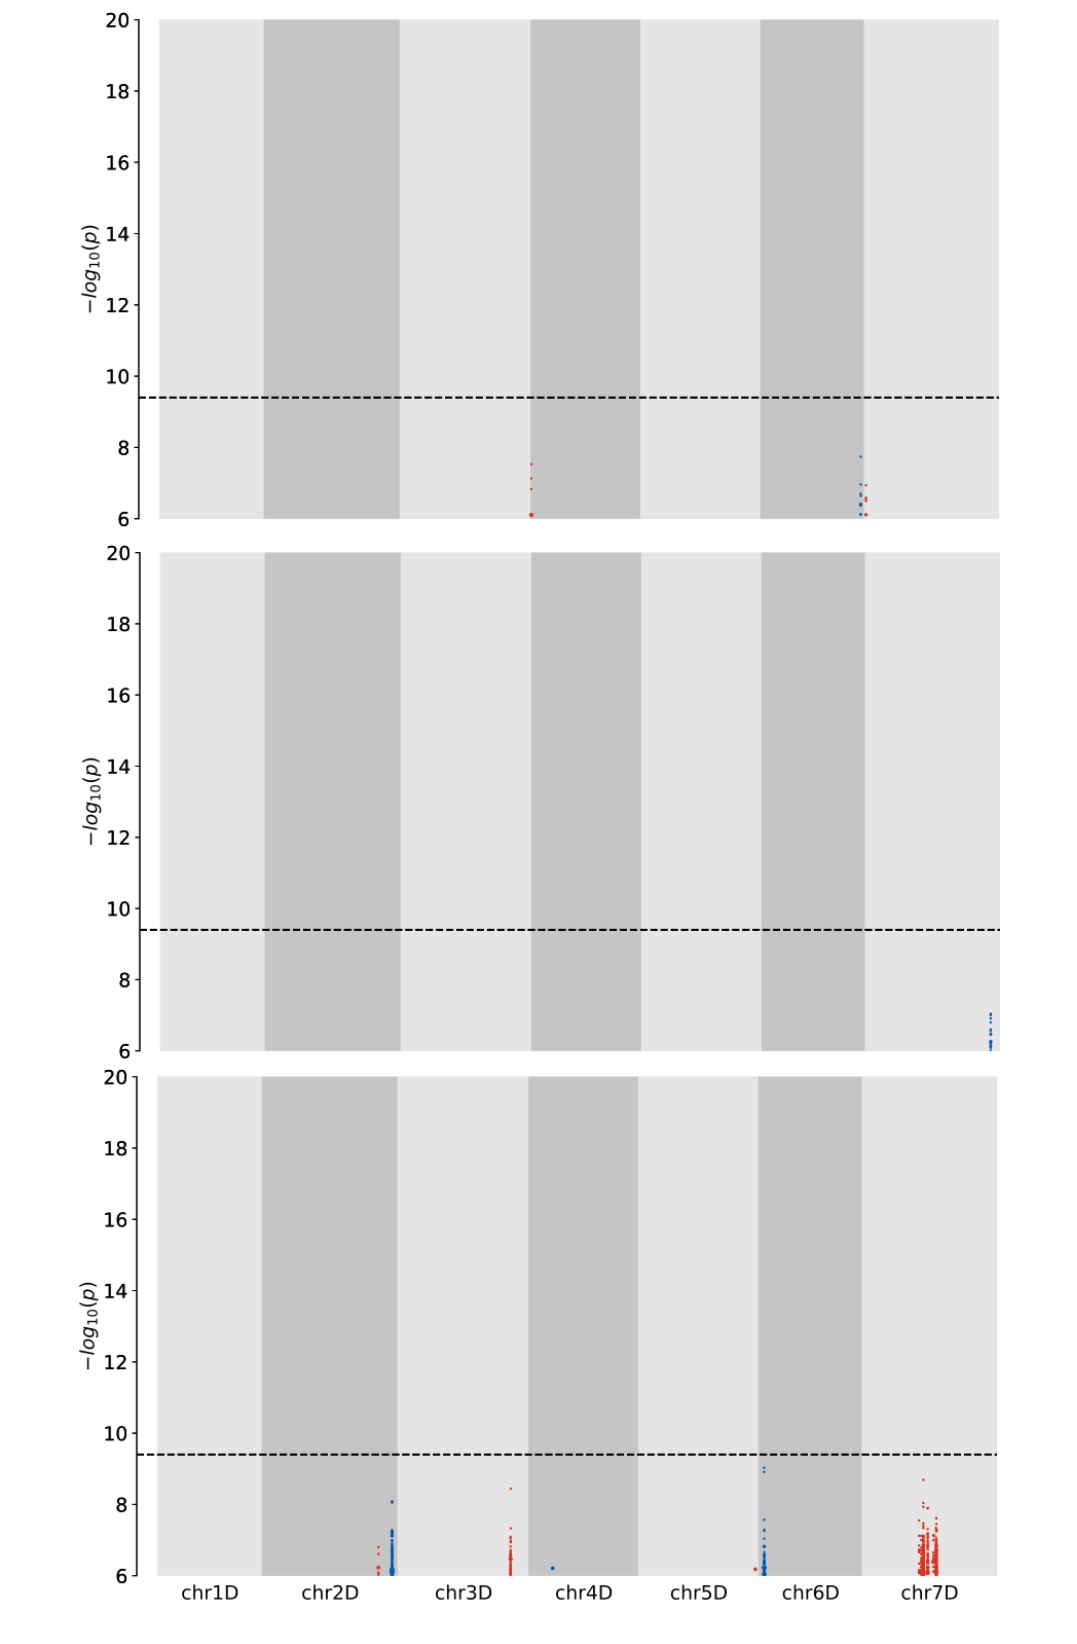
\includegraphics[width=0.8\textwidth]{images/gwas_plots/svgtopng/si_manhattan_plots.png}
        \caption{Manhattan plots of the results of our GWAS analysis for leaf silicon content in \textit{Aegilops tauschii}. Red dots indicate a negative correlation, while blue dots denote a positive correlation. The top plot shows the results for the glasshouse environment, while the bottom two plots are the outdoor environments. The dotted line represents the bonferroni-corrected significance threshold.}
        \label{Fig:si_peak_plot}
\end{figure}


\begin{figure}[h]
        \centering
        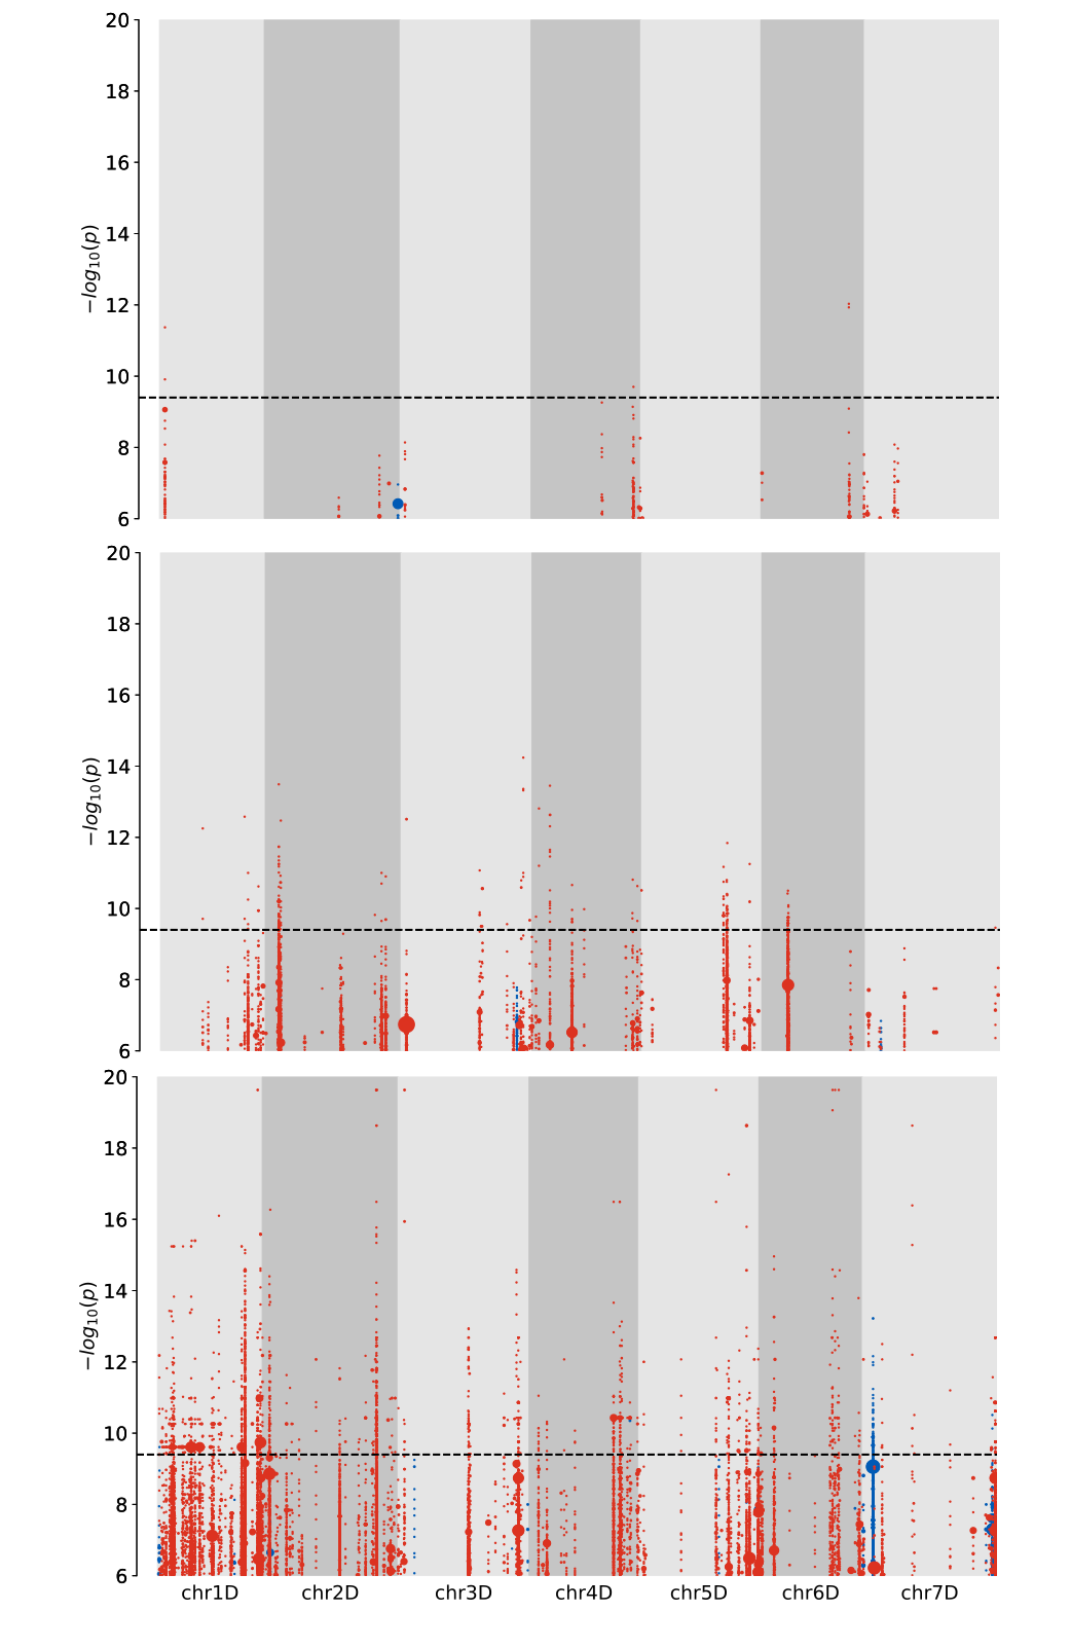
\includegraphics[width = 0.8\textwidth]{images/gwas_plots/svgtopng/mn_manhattan_plot.png}
        \label{Fig:mn_peak_plot}
        \caption{Manhattan plots of the results of our GWAS analysis for leaf manganese content in \textit{Aegilops tauschii}. Red dots indicate a negative correlation, while blue dots denote a positive correlation. The top plot shows the results for the glasshouse environment, while the bottom two plots are the outdoor environments. The dotted line represents the bonferroni-corrected significance threshold.}
\end{figure}
        

\mycomment{
\begin{figure}[h]
        \centering
        \begin{subfigure}[b]{\textwidth}
                \centering
                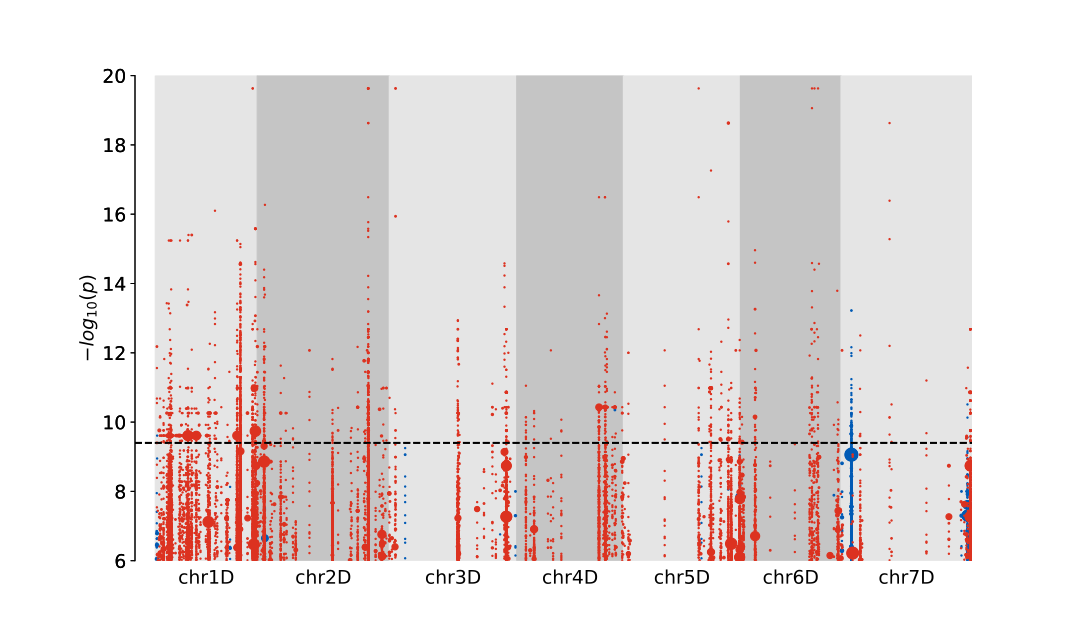
\includegraphics[scale=0.3]{images/gwas_plots/svgtopng/tf_mn_plot.png}
                \label{Fig:tf_mn_peak}
        \end{subfigure}
        \begin{subfigure}[b]{\textwidth}
                \centering
                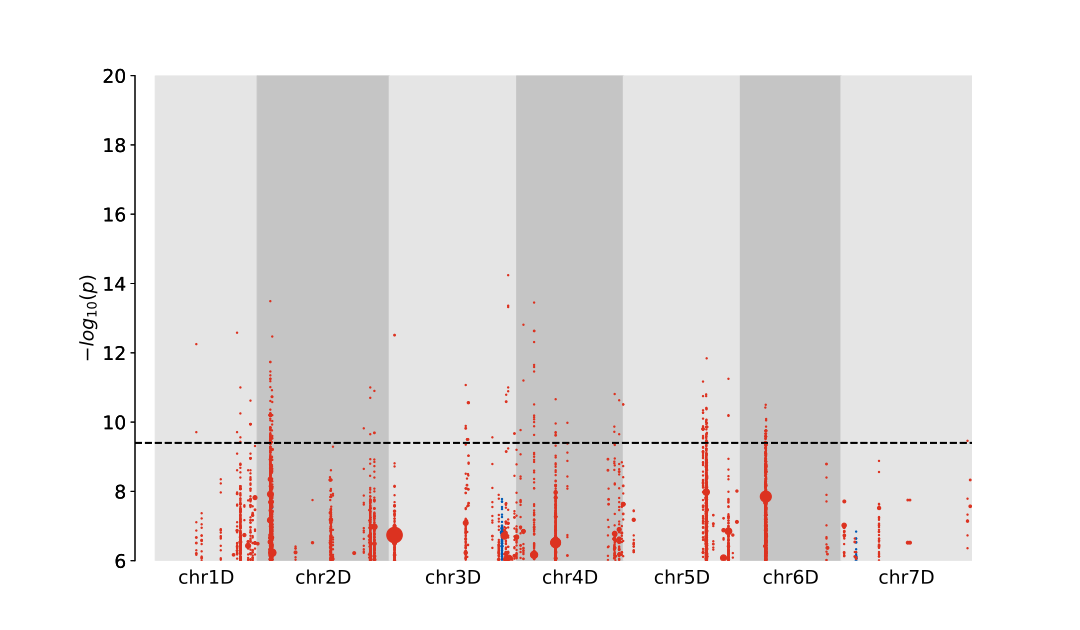
\includegraphics[scale=0.3]{images/gwas_plots/svgtopng/sc_mn_plot.png}
                \label{Fig:sc_mn_peak}
        \end{subfigure}
        \begin{subfigure}[b]{\textwidth}
                \centering
                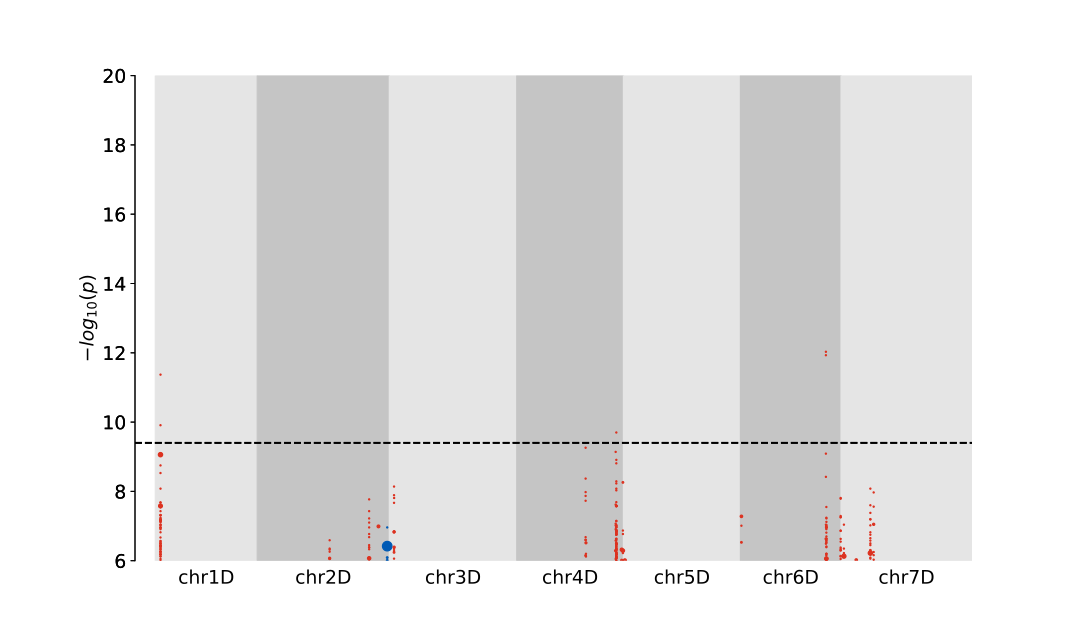
\includegraphics[scale=0.3]{images/gwas_plots/svgtopng/gh_mn_plot.png}
                \label{Fig:gh_mn_peak}
        \end{subfigure}
        \caption{Manhattan plots of the results of our GWAS analysis for leaf manganese content in \textit{Aegilops tauschii}. Red dots indicate a negative correlation, while blue dots denote a positive correlation. The top two plots show the results for the outdoor growing environments, and the bottom plot is the glasshouse environment. The dotted line represents the bonferroni-corrected significance threshold.}
        \label{Fig:mn_peak_plot_old}
\end{figure}
}

\clearpage

\chapter{Conclusion}
\section{Research Outcomes}

My aim with this thesis was to advance our understanding of how silicon-based plant traits may be applied to agriculture. To this end, I identified two separate problems that currently limit uptake and dissemination of silicon research into the broader agricultural context: 1) limited applicability of fundamental reserach into inducded silicon uptake to crop plants, and 2) a limited understanding of the genetic basis of variation in silicon content among genotypes of a common species. Based on the exciting finidngs of rapid silicon accumulation in \textit{Brachypodion distachyum}, I attemped to replicate this pattern of silicon uptake in cereal crops, in the hopes that this would spur further research into silicon-based crop defenses. In the growing conditions I used, I did not observe rapid silicon accumulation, but did observe variation in silicon and phenolic compound levels among the four crop species I tested. We also documented the significant variation among common cultivars of these cereal species.

For my GWA study, we observed significant variation in silicon and manganese content between sites. Though we failed to find robsut genotype-phenotype links for either silicon or manganese, we did identify one gene that is associated with variation in leaf manganese content. Additionally, by working with a previously developed diversity panel, we hope that our findings will be easily integrated into future work on this topic.

\section{Limitations and Future Directions}

A number of limitations with my study design and experimental methods should be noted. Though I was ultimately unsucessful in my attempts to induce rapid silicification, I identified a number of factors that could have led to the discrepancies between previous research and my own. We utilized a single herbivore species in our treatments. Plants modulate their defensive responses based on the identify of the attacker, and it is likely that using different species or multiple species would yeild different outcomes. Some of the insects in my treatments did not initiate feeding, despite our best efforts to maximise the likelihood of herbivory, and this reduced our sample size for the experiment. Finally, it is likely that the growth media we used for the study imposed some silicon limitation on our plants. This limitation may have prevented rapid uptake of silicon, as there might just not have been enough in the soil to meet the demands of the plant. Future reserach should explicitly investigate the silicon availability of commercially available plant growth media, as nearly all plants can respond positively to silicon. Additionally, we used a single time point to test for rapid silicon accumulation. It is possible that we pre-empted silicon uptake in our plants, and had we waited longer, we would have seen a clear signal of silicon uptake in response to our treatments. Future studies would provide immense utility to the field if they were to investigate silicon uptake at regular intervals between 6 and 48 hours post induction, as we still lack replicated data on this time interval. 

For the GWA study, we may have limited our ability to detect important QTLs through the use of multiple growing environments. Though multiple growing environments are often used to prove the durability of a given QTL through GxE interations, the highly exploratory nature of our work would have benefitted from a deeper and narrower experimental design, where we had more replicates in a single environment. We are left with few markers to investigate, but future work could take the genotypes we identified as having high and low silicon, and develop a mapping population using experimental crosses. The increased level of control this design would bring might allow for the discovery of QTLs associated with silicon content. Similar studies in wheat and rice have yeilded promising results, and there is no reason to believe that \textit{Aegilops tauschii} would not have similar genes that influence silicon uptake.

\end{document}